\section{Numerical solutions}\label{numerical}
In this section we numerically solve the linear stability problem
corresponding to Eq. \ref{lin_mass}---\ref{lin_energy}. 
We relax the  low-frequency, nearly-Keplerian and thin-disk 
approximations used in the analytical discussion above. We 
use the full expressions of $\rho$, $\Omega$ and 
$\kappa$ and $c_s$ given in \S\ref{eqm}. We also set $\hat{g}_c=1$ to  
account for the background radial disk structure.  

We solve the linear problem by expanding the
perturbations in Chebyshev polynomials $T_l$ up to $l=512$
and discretizing the equations on a grid with
$z\in[-\zmax,\zmax]$. Our standard boundary conditions at the vertical
boundaries is a free surface, 
\begin{align}
  \Delta P \equiv \delta P + \bm{\xi}\cdot\nabla P= 0 \quad \text{at } z=\pm\zmax,
\end{align}
%note that there are g_c terms in the boundary condition
where $\bm{\xi}$ is the Lagrangian displacement with meridional 
components $\xi_{x,z} = \ii\delta v_{x,z}/\sigma$. In some cases we
impose a rigid boundary at which $\delta v_z=0$. 

The above discretization procedure
converts the linear system of differential equations to a set of 
algebraic equations, for which we use matrix routines in the LAPACK
package to solve. 

Unless otherwise stated, our fiducial disk model is a nearly 
vertically isothermal disk with $\Gamma=1.011$, stable
stratification $\gamma=1.4$, $(p,q,\epsilon)=(-1.5,-1,0.05)$, and 
vertical domain size $\zmax=5H$. In Fig. \ref{omega_z} we plot the
corresponding equilibrium rotation profile, which shows that $\Omega$
decreases slightly away from the mid-plane.  

\begin{figure}
  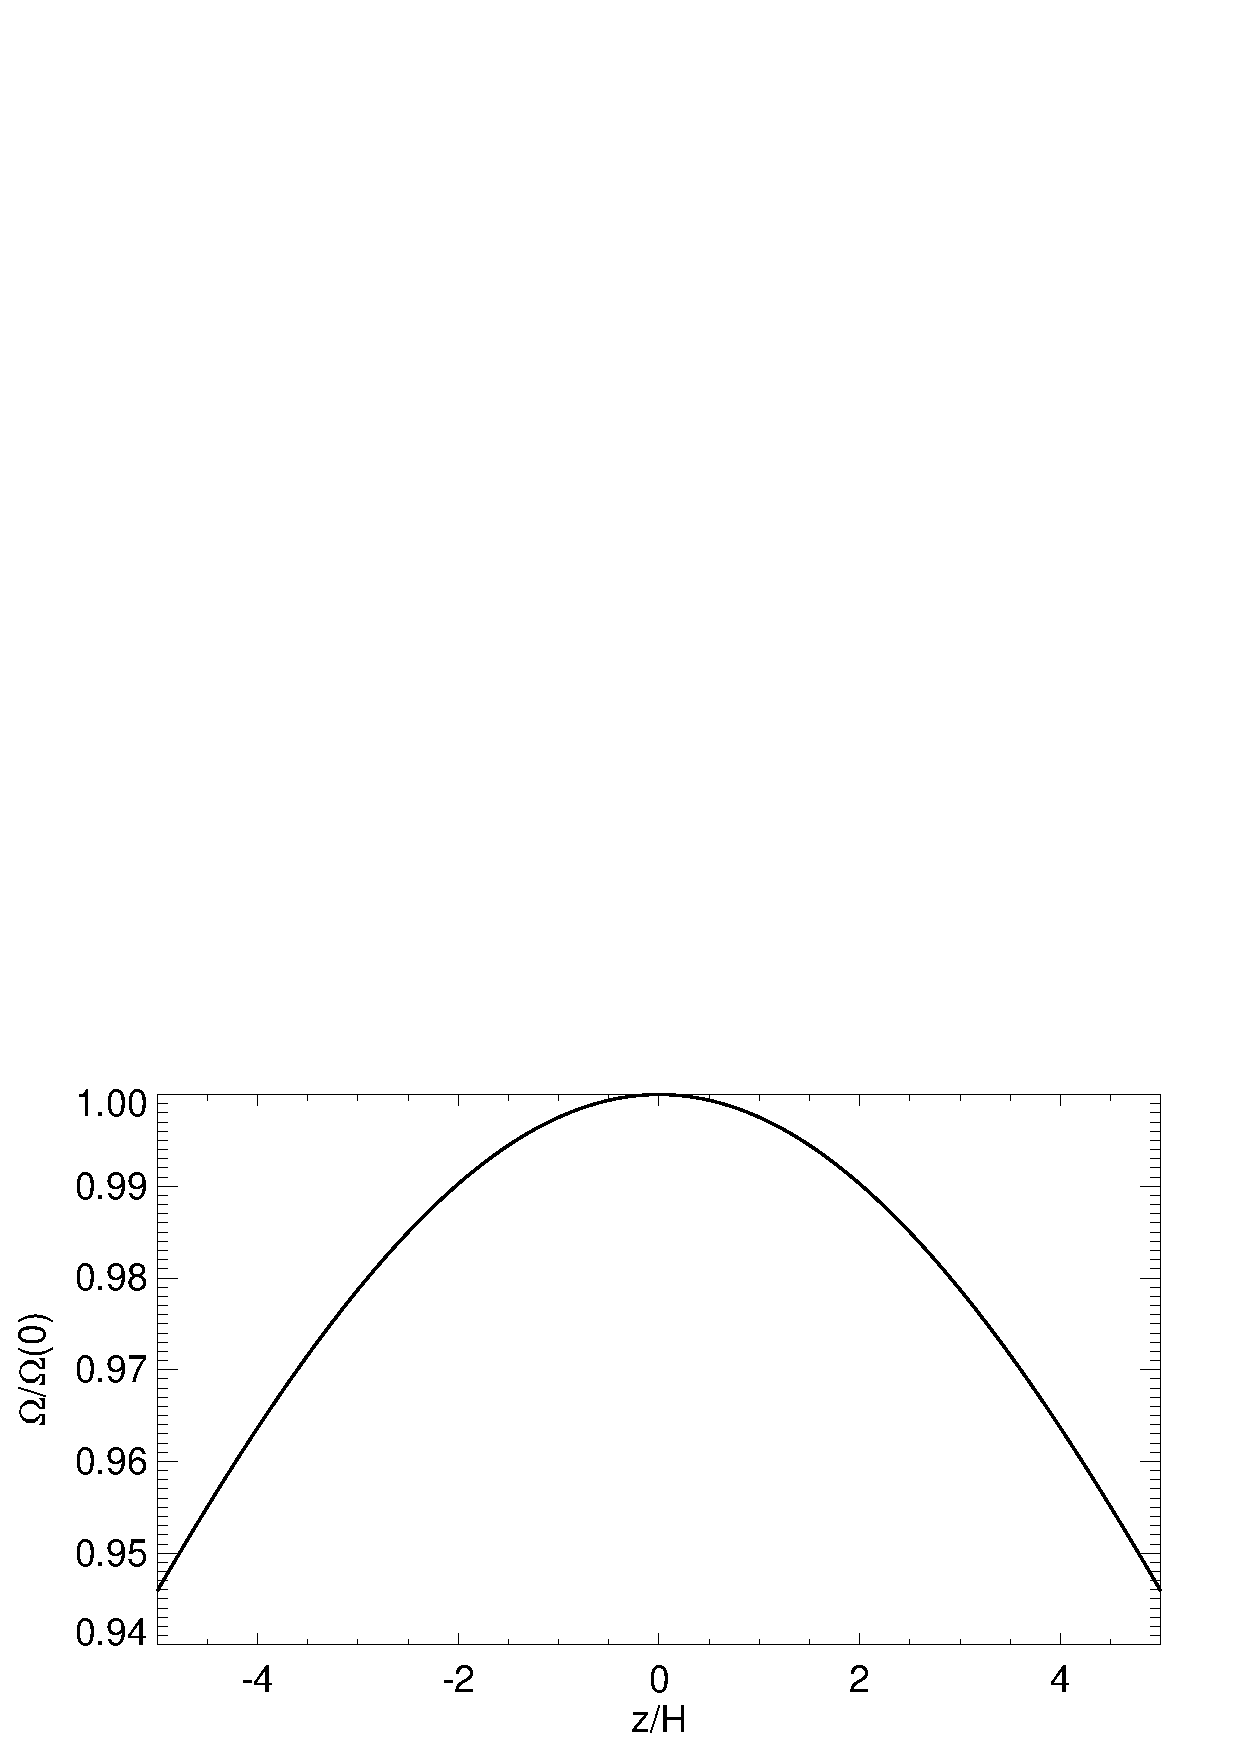
\includegraphics[width=\linewidth,clip=true,trim=0cm 0cm 0cm
  0cm]{figures/omega2} 
  \caption{Equilibrium rotation profile $\Omega(z)$,
    normalized by its mid-plane value, for a disk with $\Gamma=1.011$
    and $(p,q,\epsilon)=(-1.5,-1,0.05)$. 
    \label{omega_z} 
  }
\end{figure}

\subsection{VSI with rapid thermal relaxation}\label{vertiso_pertiso} 
We first calculate the VSI in a disk with rapid thermal relaxation by
setting $\beta=10^{-3}$. (Smaller values yield similar results.) This
is similar to strictly isothermal perturbations in a vertically
isothermal disk considered in \cite{nelson13} and \cite{mcnally14}. 

Fig. \ref{iso_eigen_kx} compares the numerically obtained eigenvalues 
for the fundamental mode and that calculated from 
Eq. \ref{simple_growth}. We find good agreement in the
wave frequency $\omega$ at all $\khat$ and in growth rates $\nu$ for
$\khat\gtrsim 10$. Growth rates are over-estimated by our analysis but 
are $O(\epsilon\Omega_k)$, which is consistent with the discussion in
Appendix \ref{max_growth1}. The match in $\nu$ worsens for
decreasing $\khat$ due to the neglect of global radial structure in
the analysis. Nevertheless, given the number of approximations made
in our analysis, the agreement is satisfactory. 

\begin{figure}
  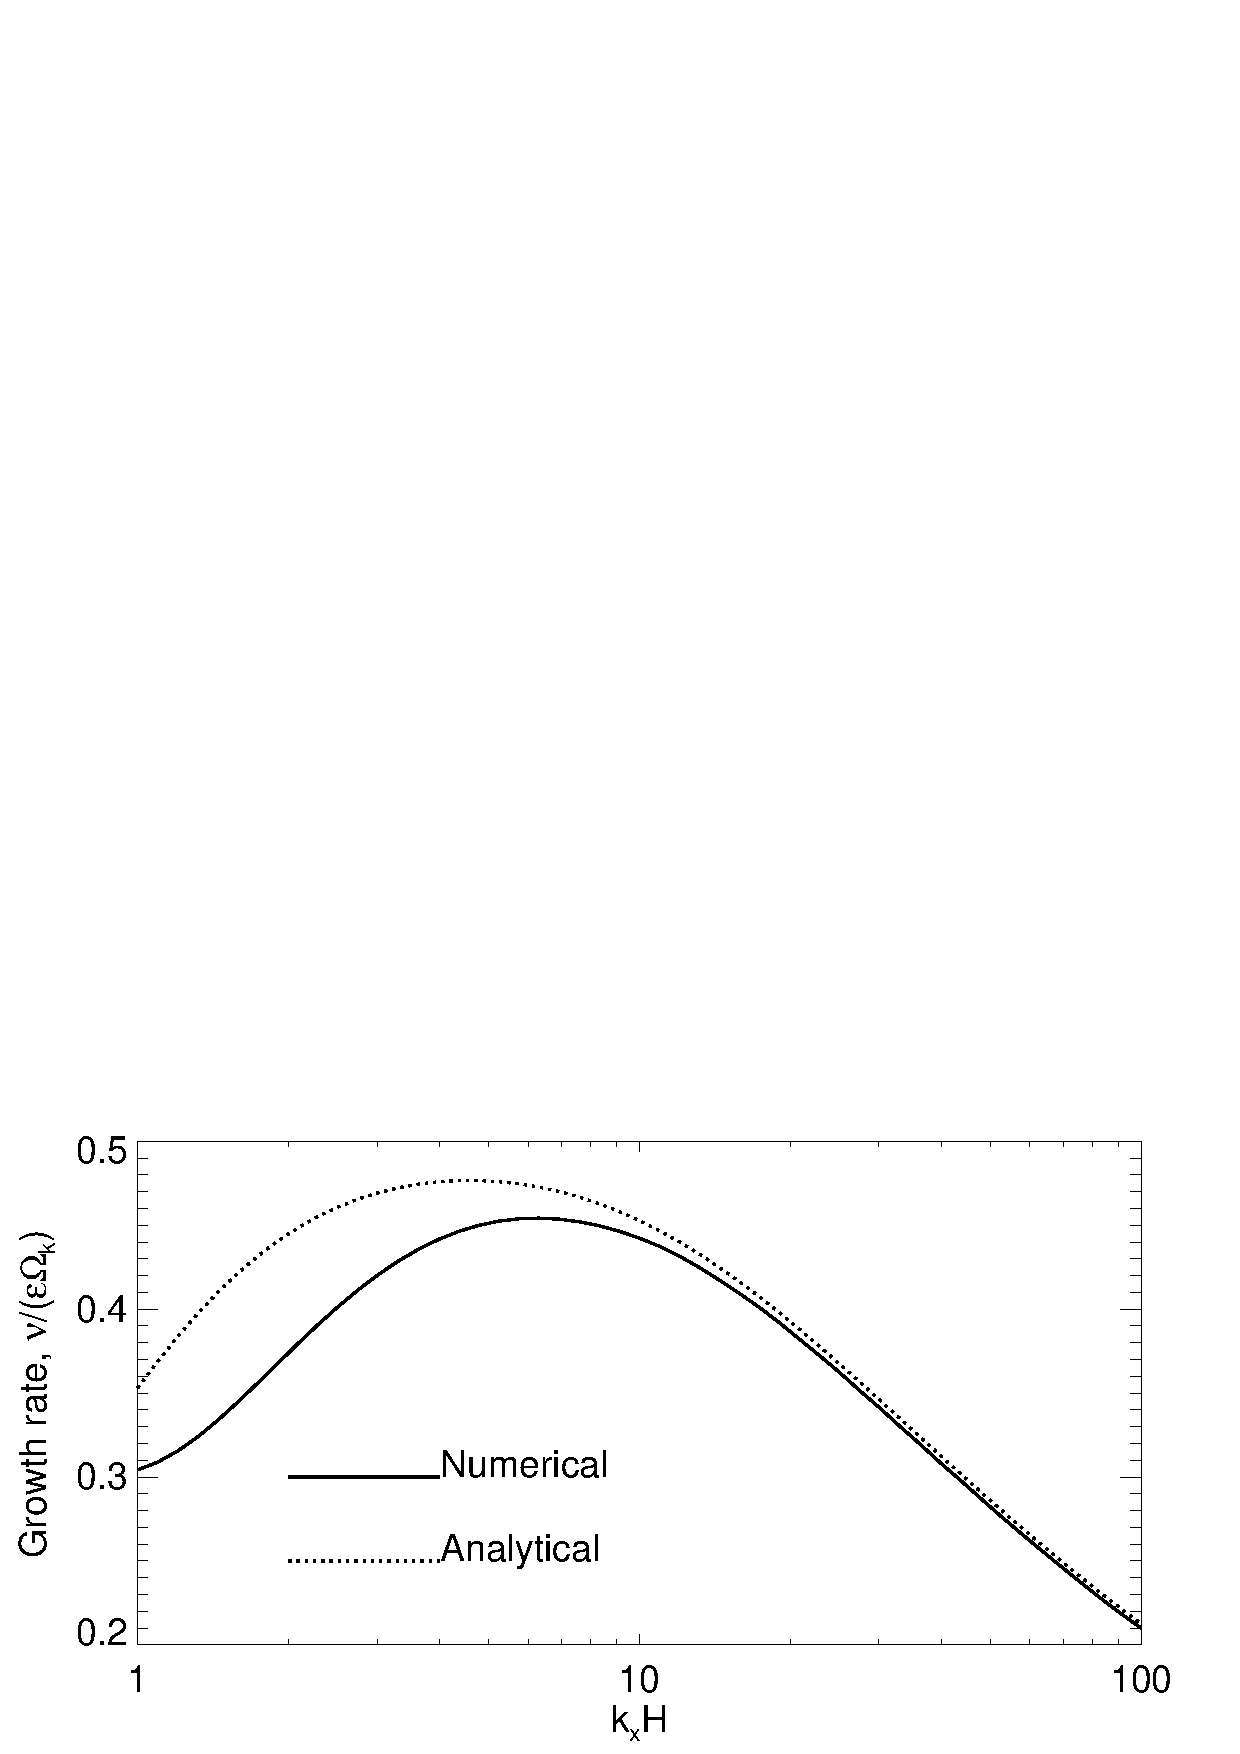
\includegraphics[width=\linewidth,clip=true,trim=0cm 1.75cm 0cm
  0cm]{figures/compare_eigen_imag_iso} 
  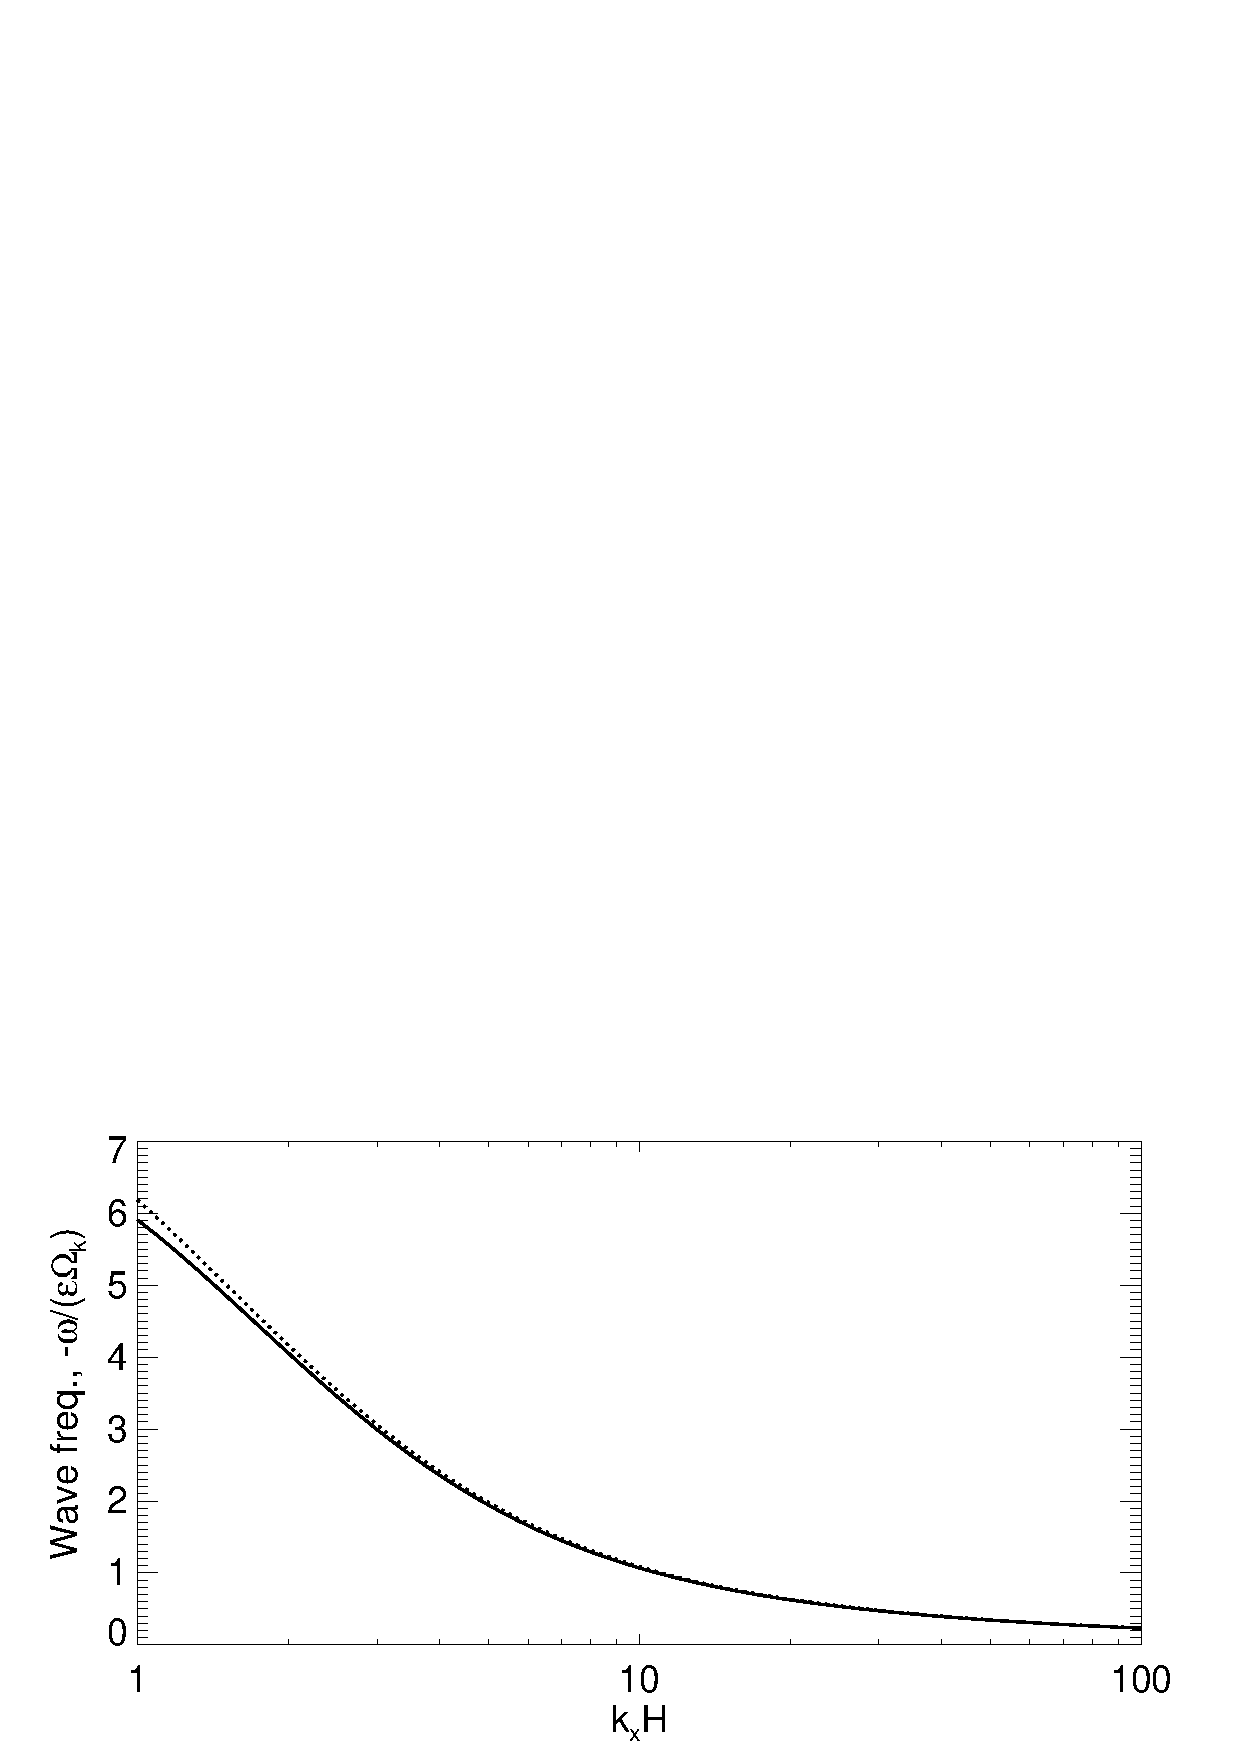
\includegraphics[width=\linewidth,clip=true,trim=0cm 0cm 0cm
  1cm]{figures/compare_eigen_real_iso}
  \caption{Growth rate (top) and real frequency (bottom) of the
    fundamental VSI mode in the fiducial disk model with $\beta =
    10^{-3}$. 
    % a disk with $(\gamma,
    % \Gamma)=(1.4,1.011)$, $(p,q,\epsilon)=(-1.5,-1,0.1)$ and
    % $\beta=10^{-3}$. 
    The solid (dotted) line is obtained numerically
    (analytically).  
    \label{iso_eigen_kx} 
  }
\end{figure}

With rapid thermal relaxation, growth rates are expected to diminish
for both $\khat\to 0$ and $\khat\to \infty$. This is because for
$\khat\ll 1$ the radial wavelength is large, but such disturbances are 
stabilized by by epicyclic motions ($|\omega|\sim
\kappa$). Disturbances with $\khat\gg 1$ are radially localized, but  
there is no energy change when fluid elements are perturbed at fixed
cylindrical radius whilst conserving its angular momentum (applicable
to axisymmetric perturbations).  
 
Fig. \ref{lowfreq_eigenfunc} plots the eigenfunctions $W$ and $\delta 
v_z$ for the fundamental mode with $\khat=10$ (i.e. the mode with
maximum growth rate in Fig. \ref{iso_eigen_kx}). We find $W\propto z$
throughout most of the disk, corresponding to a constant vertical
velocity perturbation, as expected for the fundamental mode (see
Appendix \ref{iso_explicit}). We show a meridional visualization of
this mode in Fig. \ref{lowfreq_eigenfunc_2d}. The $x$ axis is
stretched for clarity; radial velocities are in fact typically much 
smaller than vertical velocities. Most of the meridional kinetic energy is
contained within $\sim 2H$ of the midplane due to the density 
stratification. 

\begin{figure}
  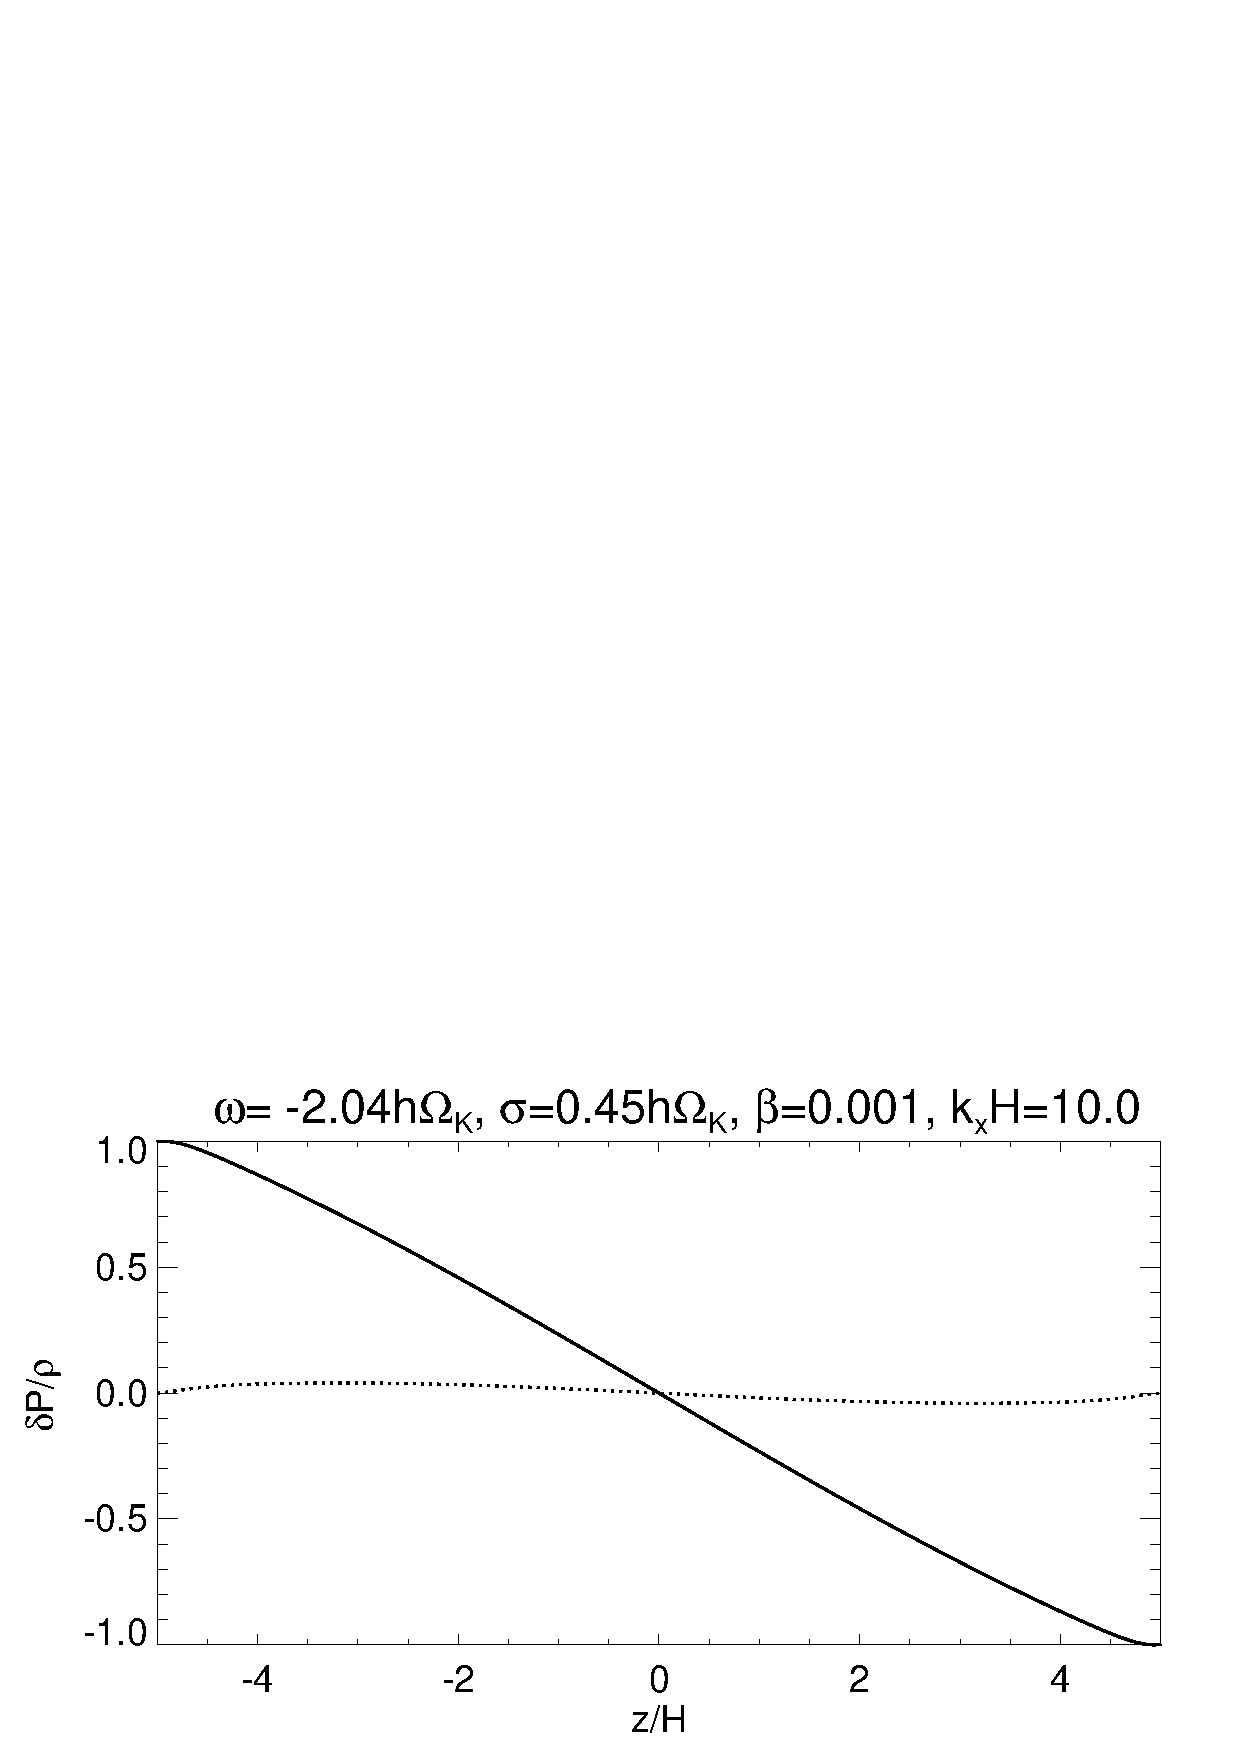
\includegraphics[width=\linewidth,clip=true,trim=0cm 1.75cm 0cm
  0cm]{figures/eigenvectorW_iso} 
  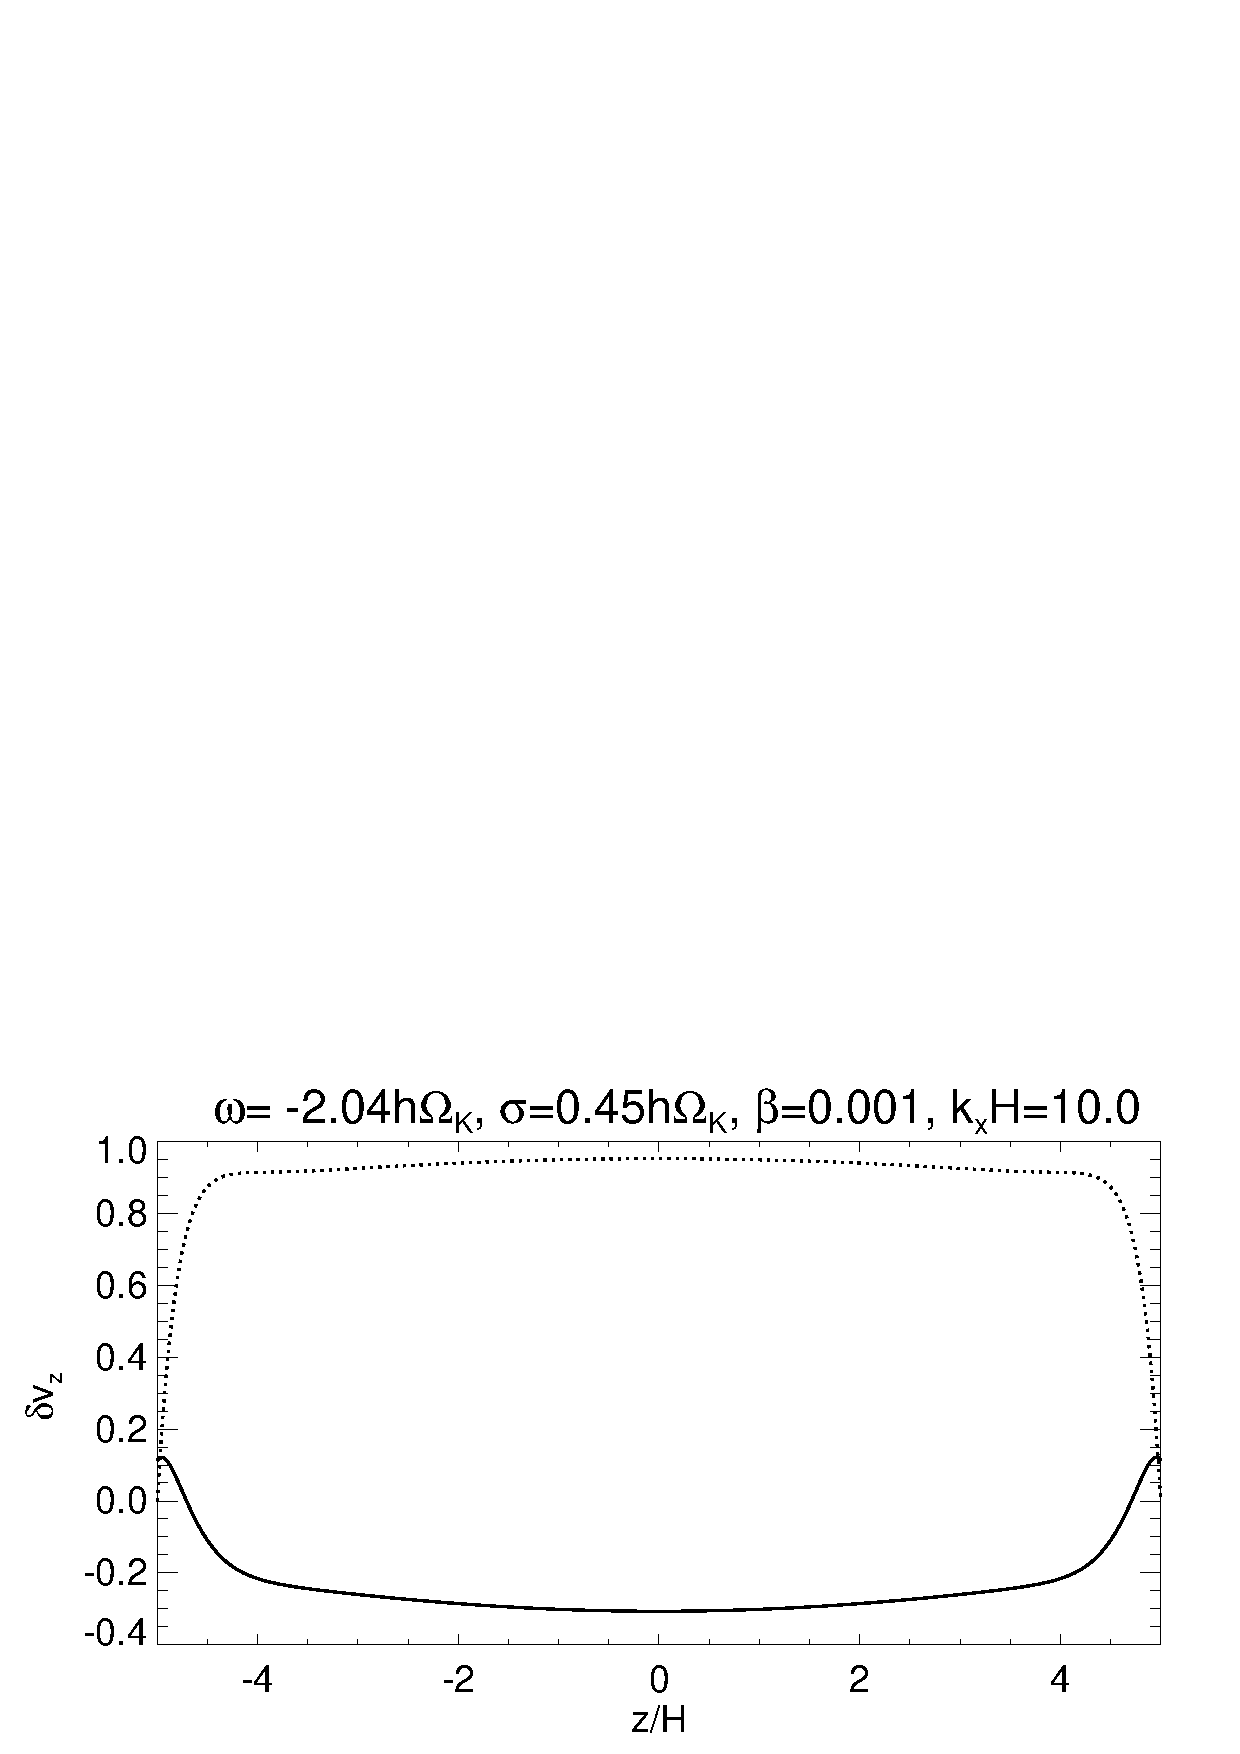
\includegraphics[width=\linewidth,clip=true,trim=0cm 0cm 0cm
  1cm]{figures/eigenvectorvz_iso}
  \caption{Pseudo-enthalpy perturbation $W$ (top) and vertical velocity
    perturbation $\delta v_z$ of the fundamental VSI with 
    $\khat=10$ in the fiducial disk with $\beta=10^{-3}$. The real 
    (imaginary) parts of $W$ and $\delta v_z$ are plotted as solid
    (dotted) lines. 
    \label{lowfreq_eigenfunc}
  }
\end{figure}


\begin{figure}
%  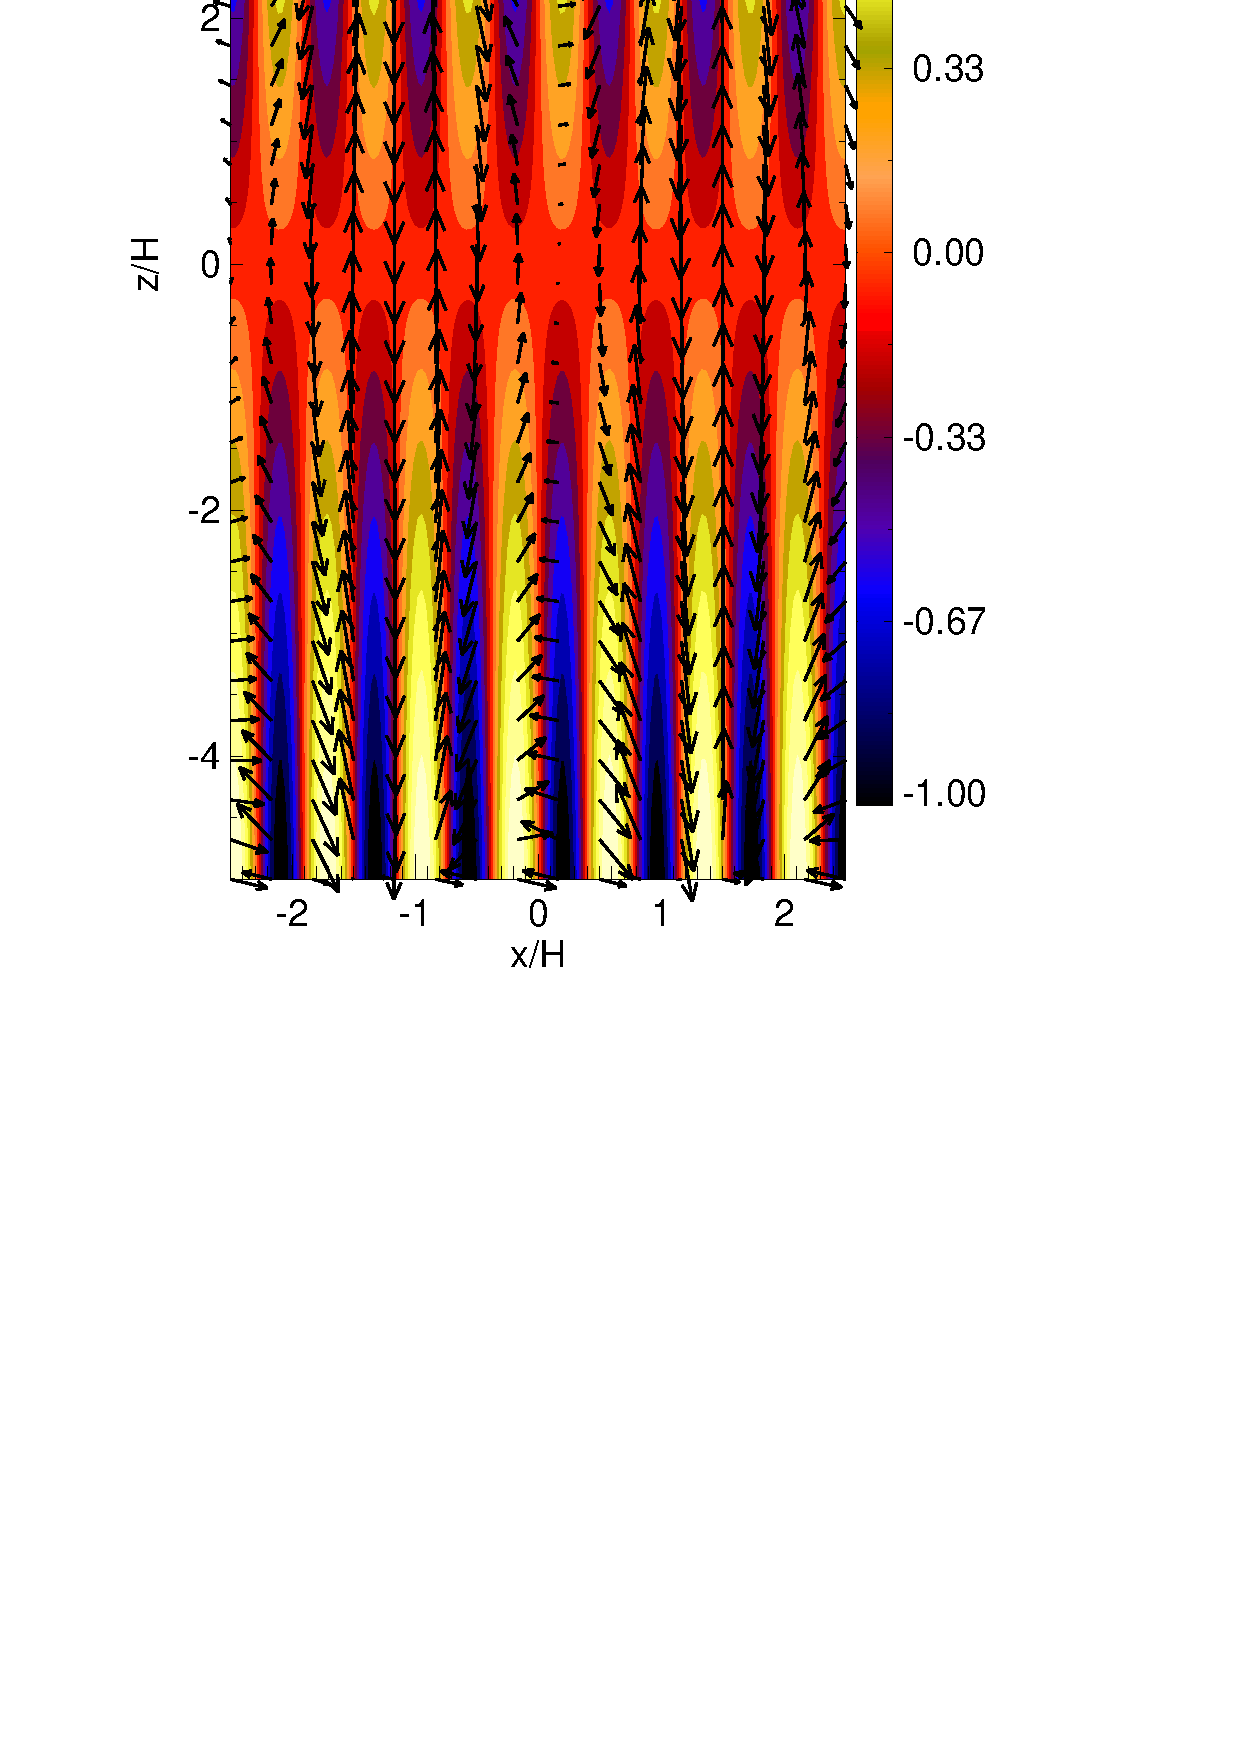
\includegraphics[scale=0.345,clip=true,trim=0cm 0cm 2.5cm
%  0cm]{figures/result2d_vel}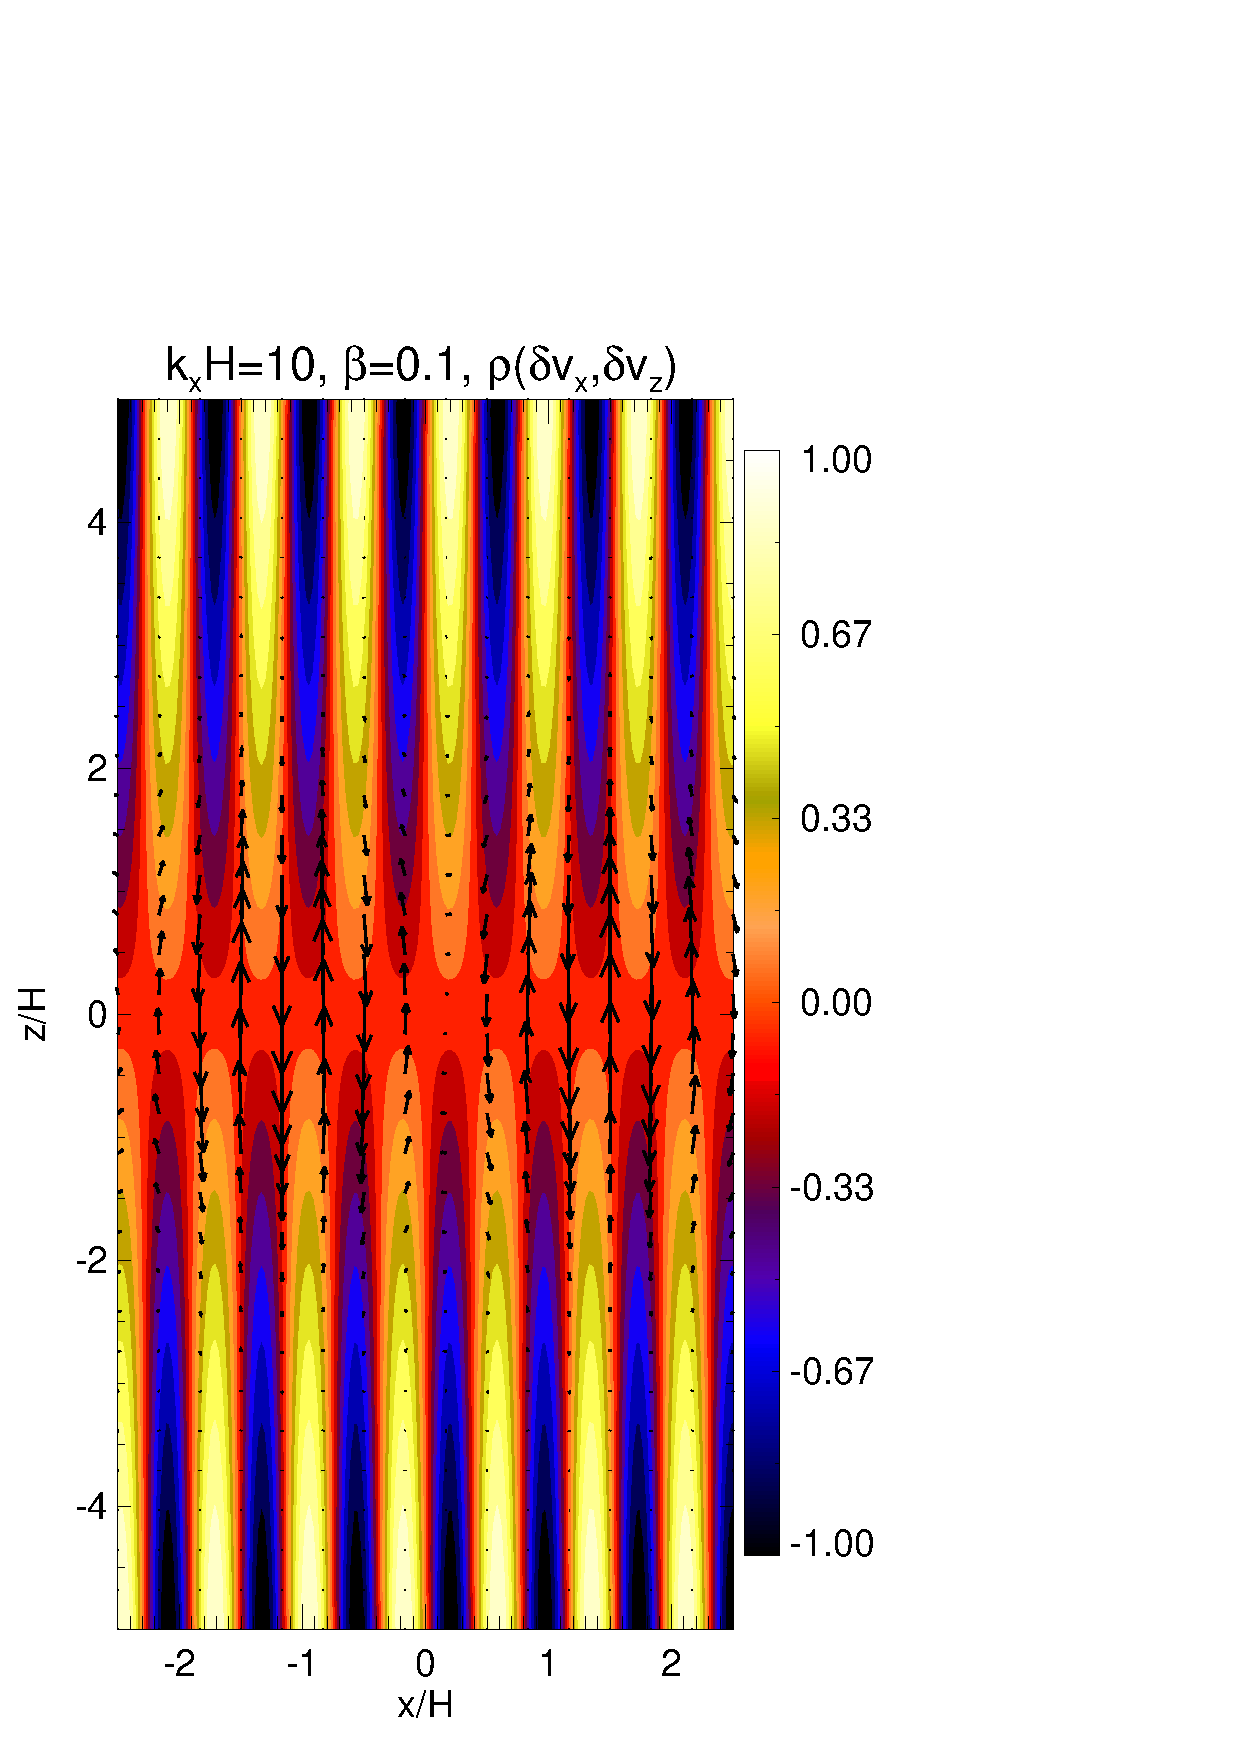
\includegraphics[scale=0.345,clip=true,trim=1.9cm 0cm 0cm
%  0cm]{figures/result2d_mom} 
  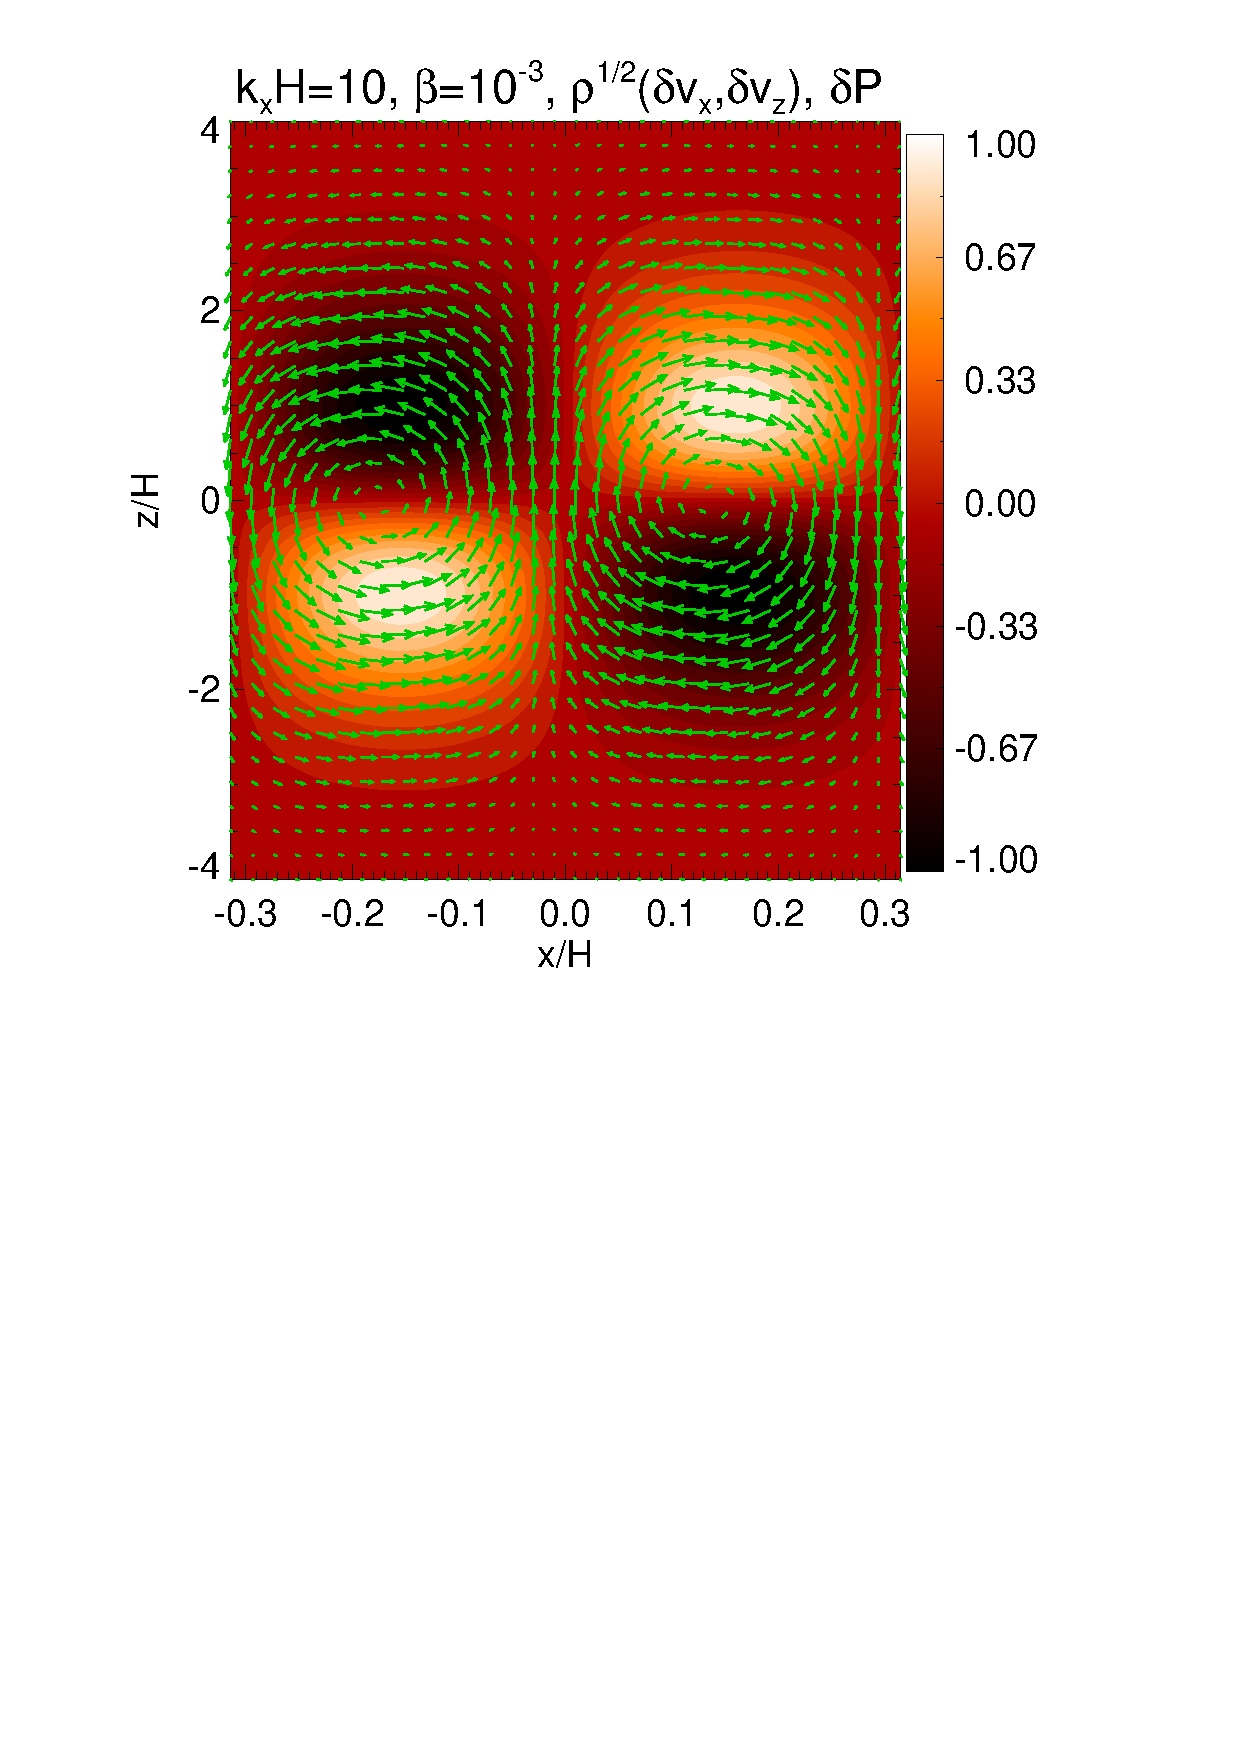
\includegraphics[width=\linewidth]{figures/result2d_iso}
  \caption{Visualization of the fundamental VSI mode in
    Fig. \ref{lowfreq_eigenfunc}. The color scale corresponds to the
    pressure perturbation $\delta P=\rho W$ scaled by its maximum value.
    Arrows correspond to the vector field field $\sqrt{\rho}(\delta
    v_x,\delta v_z)$. Note that the horizontal axis has been stretched 
    for clarity.  
    \label{lowfreq_eigenfunc_2d}
  }
\end{figure}


\subsubsection{Case study: $\khat=10$}
In Fig. \ref{compare_modes_iso_kx10} we plot eigenvalues of unstable 
modes with $\khat=10$. Black dots correspond to our fiducial setup. 
We also plot other calculations with different
vertical boundary conditions: rigid boundary and $\zmax=5H$ (red
crosses),  free surface and $\zmax = 3H$ (blue triangles), free surface
and $\zmax=7H$ (green crosses). 

The fundamental mode, marked by `f', corresponds to the eigenvalue
with the smallest $|\sigma|$. The fundamental mode is
robust against the vertical boundary conditions considered as it
appears at the same position in all cases. Higher order modes along
the analytic lines have larger growth rates, but require larger
vertical domains, since they have increasing number of nodes  $z$.  

The `tail' end of modes with decreasing $\nu$ to the right of
Fig. \ref{compare_modes_iso_kx10} is not predicted by our 
analysis. They have lower growth rates than modes consistent with our
analysis (i.e. those along the lines). These modes differ significantly between
cases and are thus likely associated with boundary conditions. % We do
                                % not consider them  
                                % further.  

\begin{figure}
  \includegraphics[width=\linewidth]{figures/compare_modes_iso_kx10_analytic.ps}
  \caption{Unstable modes with $\khat=10$ in the fiducial disk model
    with $\beta=10^{-3}$. %  a disk with 
    % $(\gamma,\Gamma)=(1.4,1.011)$, $(p,q,\epsilon)=(-1.5,-1,0.1)$ and
    % $\beta=10^{-3}$. 
    The fiducial boundary condition is a free surface ($\Delta P=0$)
    with vertical domain size $\zmax=5H$  (black dots).  Other
    cases correspond to different boundary conditions applied at
    different heights. The fundamental mode is marked by `f'. Lines
    are computed from the analytic dispersion relation 
    with thermal relaxation Eq. \ref{relax_disp} (dotted), and that for
    isothermal perturbations, Eq. \ref{simple_growth} (dashed). 
    \label{compare_modes_iso_kx10} 
  }
\end{figure}

\subsubsection{Comment on `surface modes'}\label{surf_comment}
Our fiducial setup with $\khat=10$ in 
Fig. \ref{compare_modes_iso_kx10} (black dots) differs to that from
\cite{nelson13} and \cite{mcnally14} in the lack of `surface modes'. 
These modes lie almost parallel to the vertical axis in mode 
diagrams such as Fig. \ref{compare_modes_iso_kx10}. We find them for 
sufficiently large $\zmax$ and/or $\khat$. 

To illustrate this, we plot the mode diagram for $\khat=30$ in  
Fig. \ref{compare_modes_iso_kx30} with different boundary 
conditions. Surface modes are readily identified for 
$\zmax\geq 5H$ and are marked by `s'. They have the largest growth
rates but require sufficiently large vertical domain size and their
eigenvalues vary with $\zmax$.   

Due to their dependence on boundary conditions, we do not consider
surface modes further in detail, which have
already been discussed in the aforementioned studies. In fact, we will
see in the next section that surface modes are more effectively
stabilized by finite thermal relaxation than the fundamental mode. 

\begin{figure}
  \includegraphics[width=\linewidth]{figures/compare_modes_iso_kx30_analytic.ps}
  \caption{Same as Fig. \ref{compare_modes_iso_kx10} but for $\khat=30$. Examples of surface modes are
    marked by `s'. \label{compare_modes_iso_kx30}
  }
\end{figure}


\subsection{Effect of thermal relaxation}\label{therm_relax_eff}
We now consider the effect of finite thermal relaxation by increasing 
$\beta$. Note that for the fiducial disk model the critical thermal 
timescale $\beta_\mathrm{crit} = 0.125$.  

Fig. \ref{compare_modes_cool_kx10} show unstable modes with $\khat=10$ 
and $\beta\in[0.01,0.1]$. In addition to our fiducial setup with 
$\zmax=5H$, we also plot results for $\zmax=3H$, $\zmax=7H$ and 
analytic results computed from Eq. \ref{relax_disp}.  %analytic
                                %results for low order modes

We find the number of unstable modes decrease with increasing
$\beta$. Consider the fiducial setup with $\zmax=5H$ 
(middle panel). The fundamental mode ($M=0$) is not the most unstable for   
$\beta=0.01$ as there are modes with $M>0$ that have larger growth 
rates. However, by comparing with results for $\zmax=3H$, we see these
higher order modes are strongly influenced by boundary conditions, and
there is a significant mismatch between numerical and analytical
results for $\zmax=3H$ for $M>1$.   

However, the fundamental mode is dominant for $\beta \geq 
0.03$. Higher order modes, with larger growth rates at small $\beta$,
are more effectively stabilized with increasing $\beta$. For
$\beta=0.1$, which is close to $\beta_\mathrm{crit}$, we only find the
fundamental mode. This is consistent with the discussion in 
\S\ref{iso_vsi_beta_crit}.    

\begin{figure}
  \includegraphics[width=\linewidth,clip=true,trim=0cm 1.75cm 0cm
  0cm]{figures/compare_modes_cool_kx10_z3_analytic.ps} 
  \includegraphics[width=\linewidth,clip=true,trim=0cm 1.75cm 0cm
  0cm]{figures/compare_modes_cool_kx10_z5_analytic.ps}
  \includegraphics[width=\linewidth]{figures/compare_modes_cool_kx10_z7_analytic.ps}
  \caption{Unstable modes with $\khat=10$ and thermal
    relaxation timescales $\beta=0.01$ (black dots), $\beta=0.03$ (red
    crosses), $\beta=0.05$ (blue triangles) and $\beta=0.1$ (green 
    crosses); for different vertical domain sizes $\zmax=3H$ (top),
    $\zmax=5H$ (middle, the fiducial setup) and $\zmax=7H$
    (bottom). Lines are computed from
    Eq. \ref{relax_disp} for  $M=0$ (solid, fundamental mode) and
    $M=1,\,2,\,3$ (dotted, dashed, dash-dot, respectively). Along each
    line, $\beta$ increases continuously from $0.01$ to $0.1$ from top
    to bottom, and squares mark corresponding $\beta$ values with
    numerical results. 
    \label{compare_modes_cool_kx10} 
  }
\end{figure}

Fig. \ref{lowfreq_eigenfunc_cool}---\ref{lowfreq_eigenfunc_2d_cool}
shows the fundamental mode with $\khat=10$ in a disk with 
$\beta=0.1$. Comparing these plots with
Fig. \ref{lowfreq_eigenfunc}---\ref{lowfreq_eigenfunc_2d}, which have
$\beta=10^{-3}$, we see that increasing $\beta$ restricts the region 
characterized by $W\sim z$ and $\delta v_z\sim$ constant closer to the
mid-plane, with oscillatory behavior emerging near vertical boundaries
where buoyancy becomes important. This leads to the `tilted' pressure
perturbations seen in Fig. \ref{lowfreq_eigenfunc_2d_cool} 
(cf. Fig. \ref{lowfreq_eigenfunc_2d}). 

\begin{figure}
  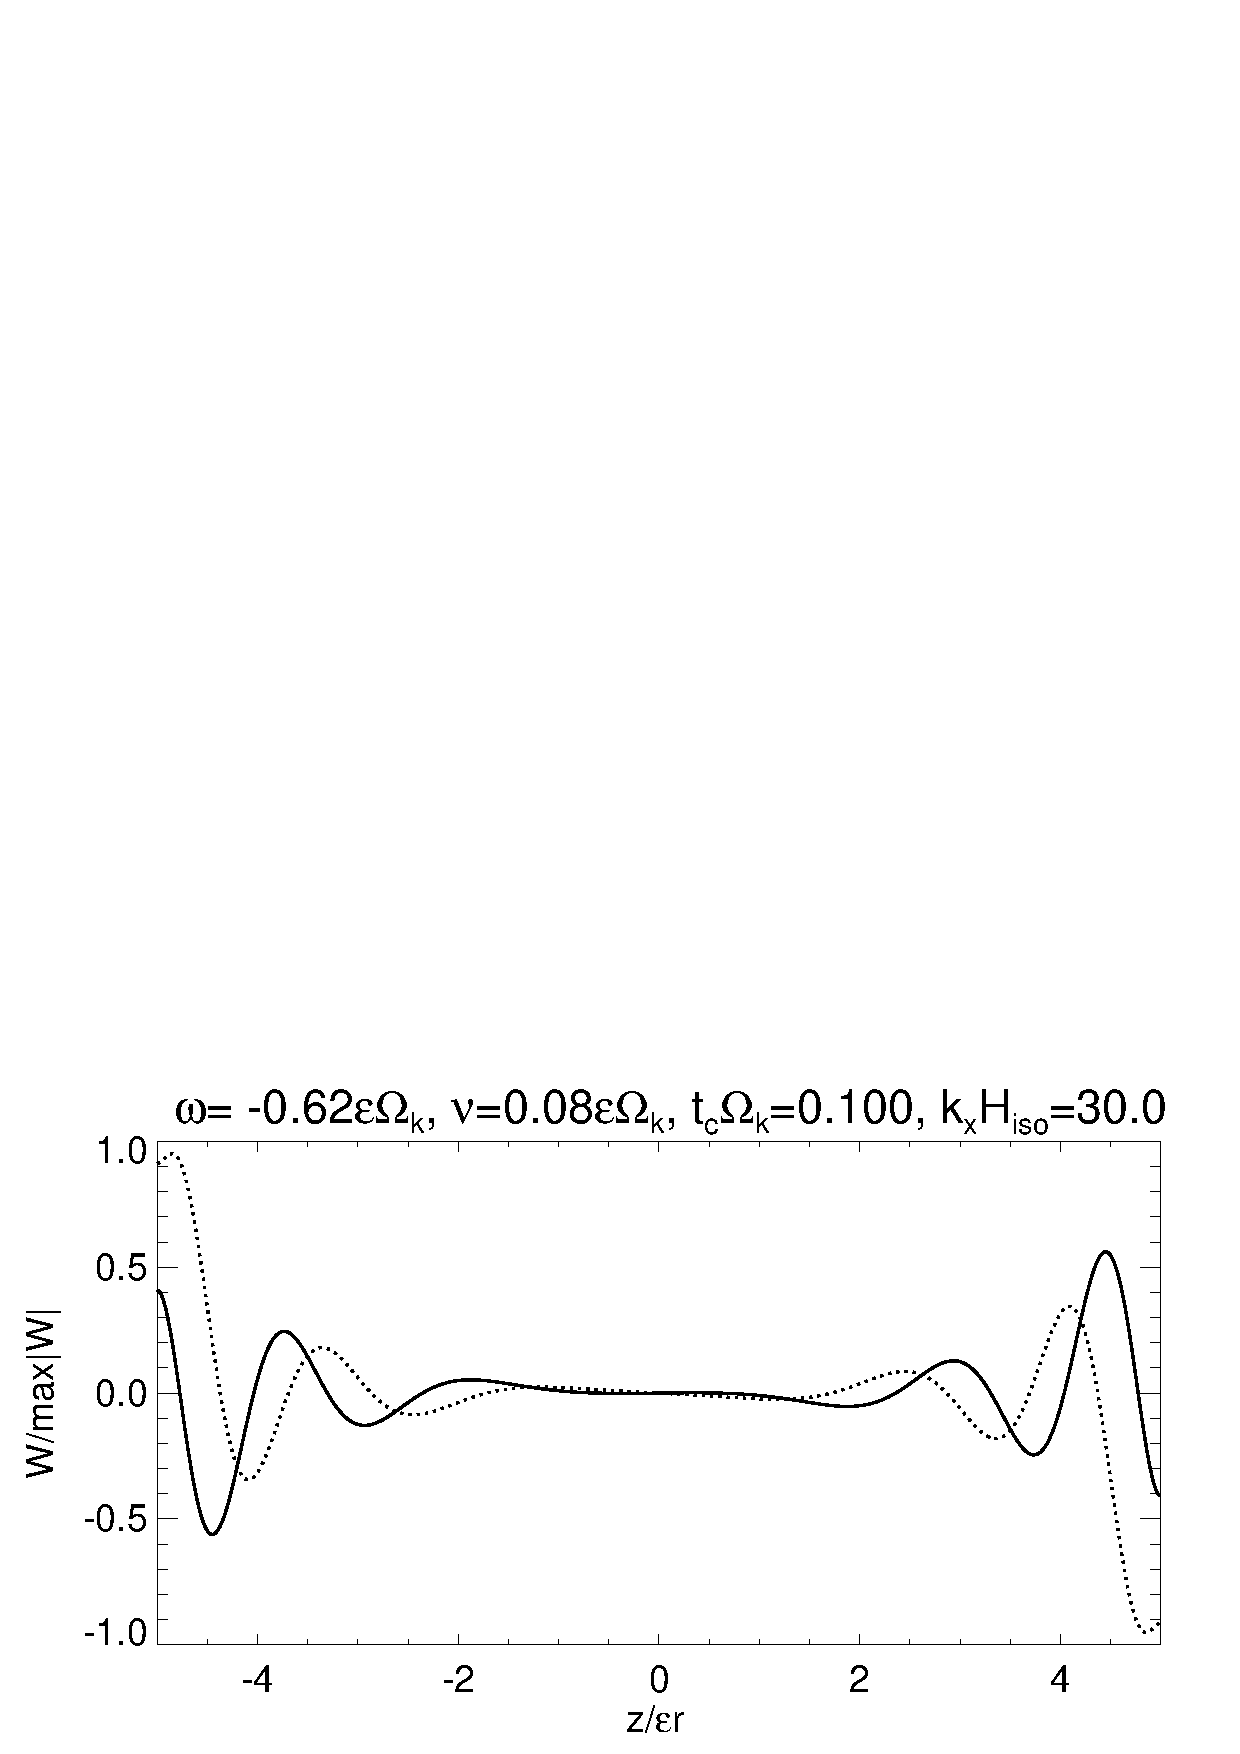
\includegraphics[width=\linewidth,clip=true,trim=0cm 1.75cm 0cm
  0cm]{figures/eigenvectorW_beta0d1} 
  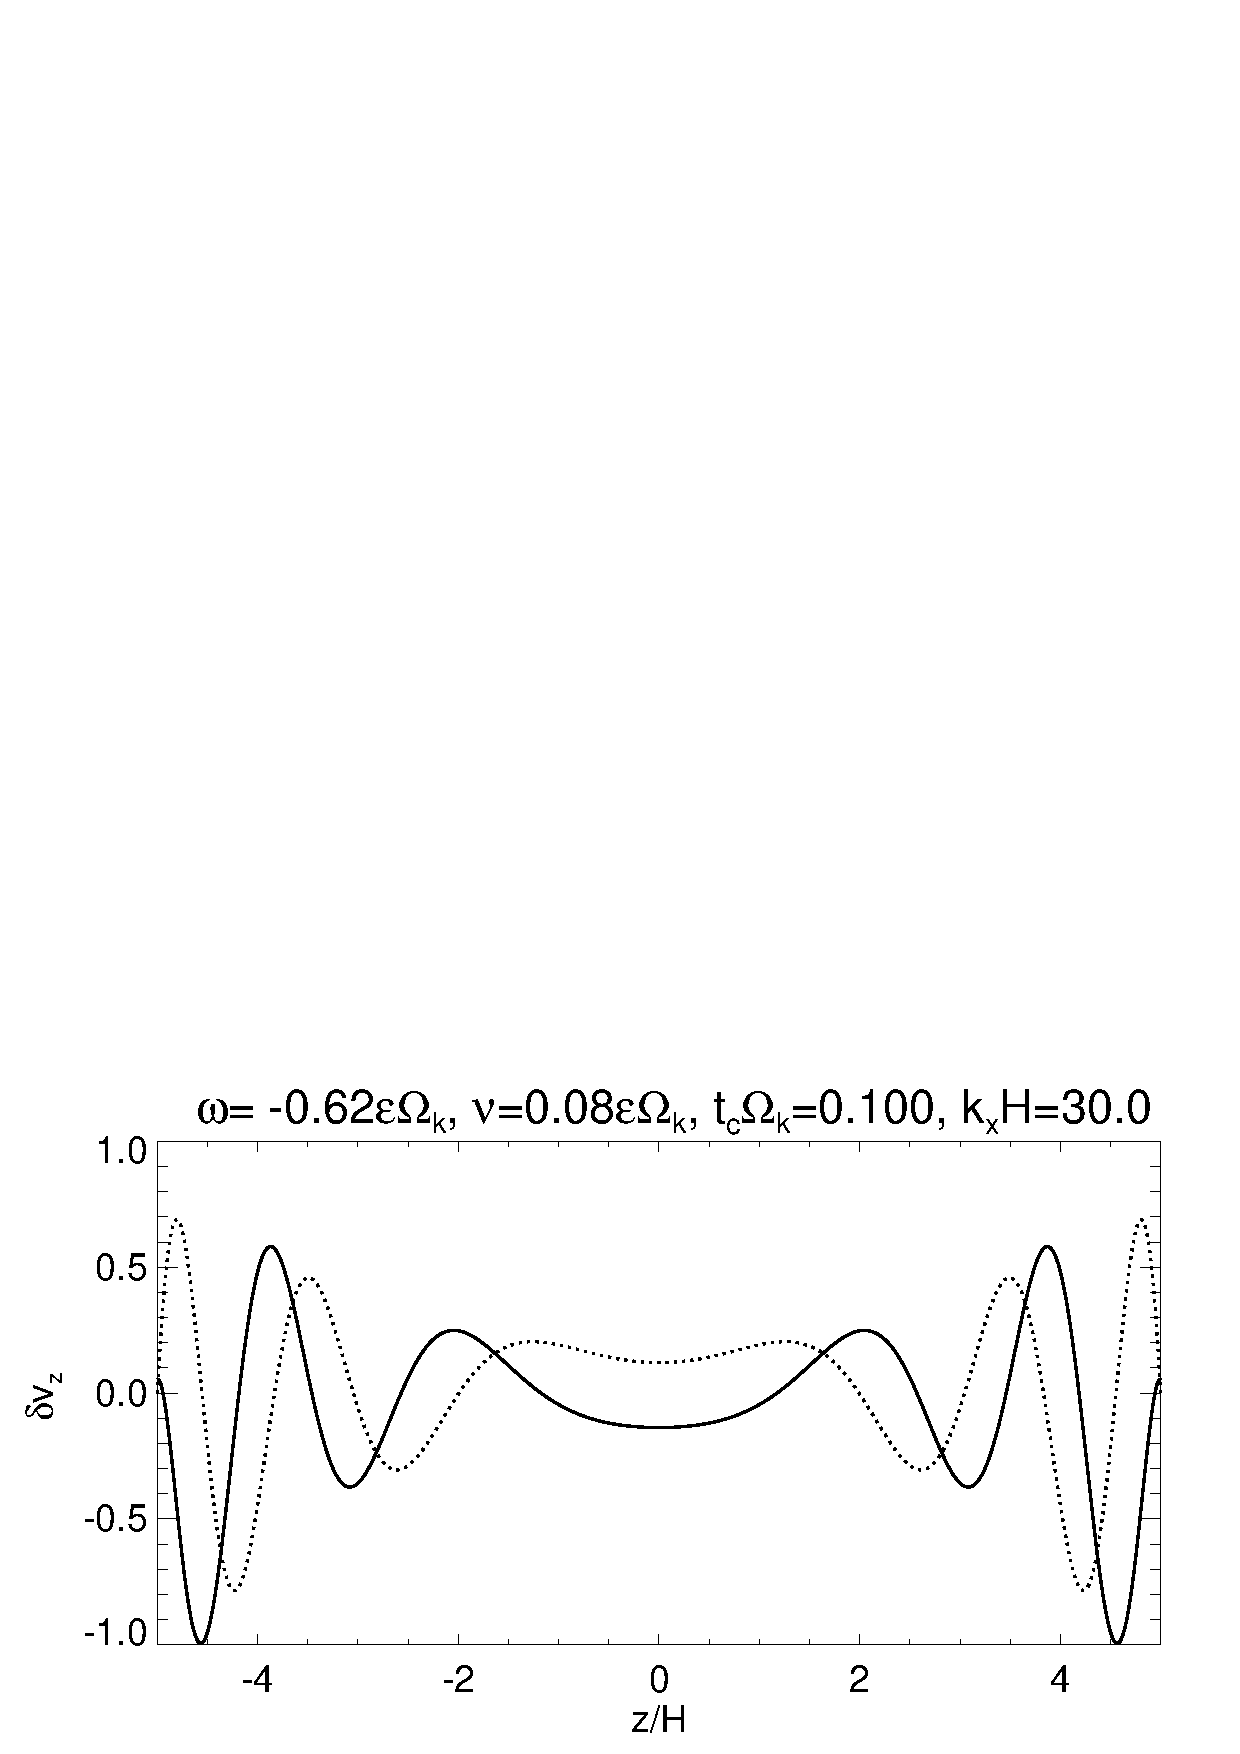
\includegraphics[width=\linewidth,clip=true,trim=0cm 0cm 0cm
  1cm]{figures/eigenvectorvz_beta0d1}
  \caption{Same as Fig. \ref{lowfreq_eigenfunc} but with a
    thermal relaxation timescale $\beta=0.1$. 
    \label{lowfreq_eigenfunc_cool}
  }
\end{figure}

\begin{figure}
  % 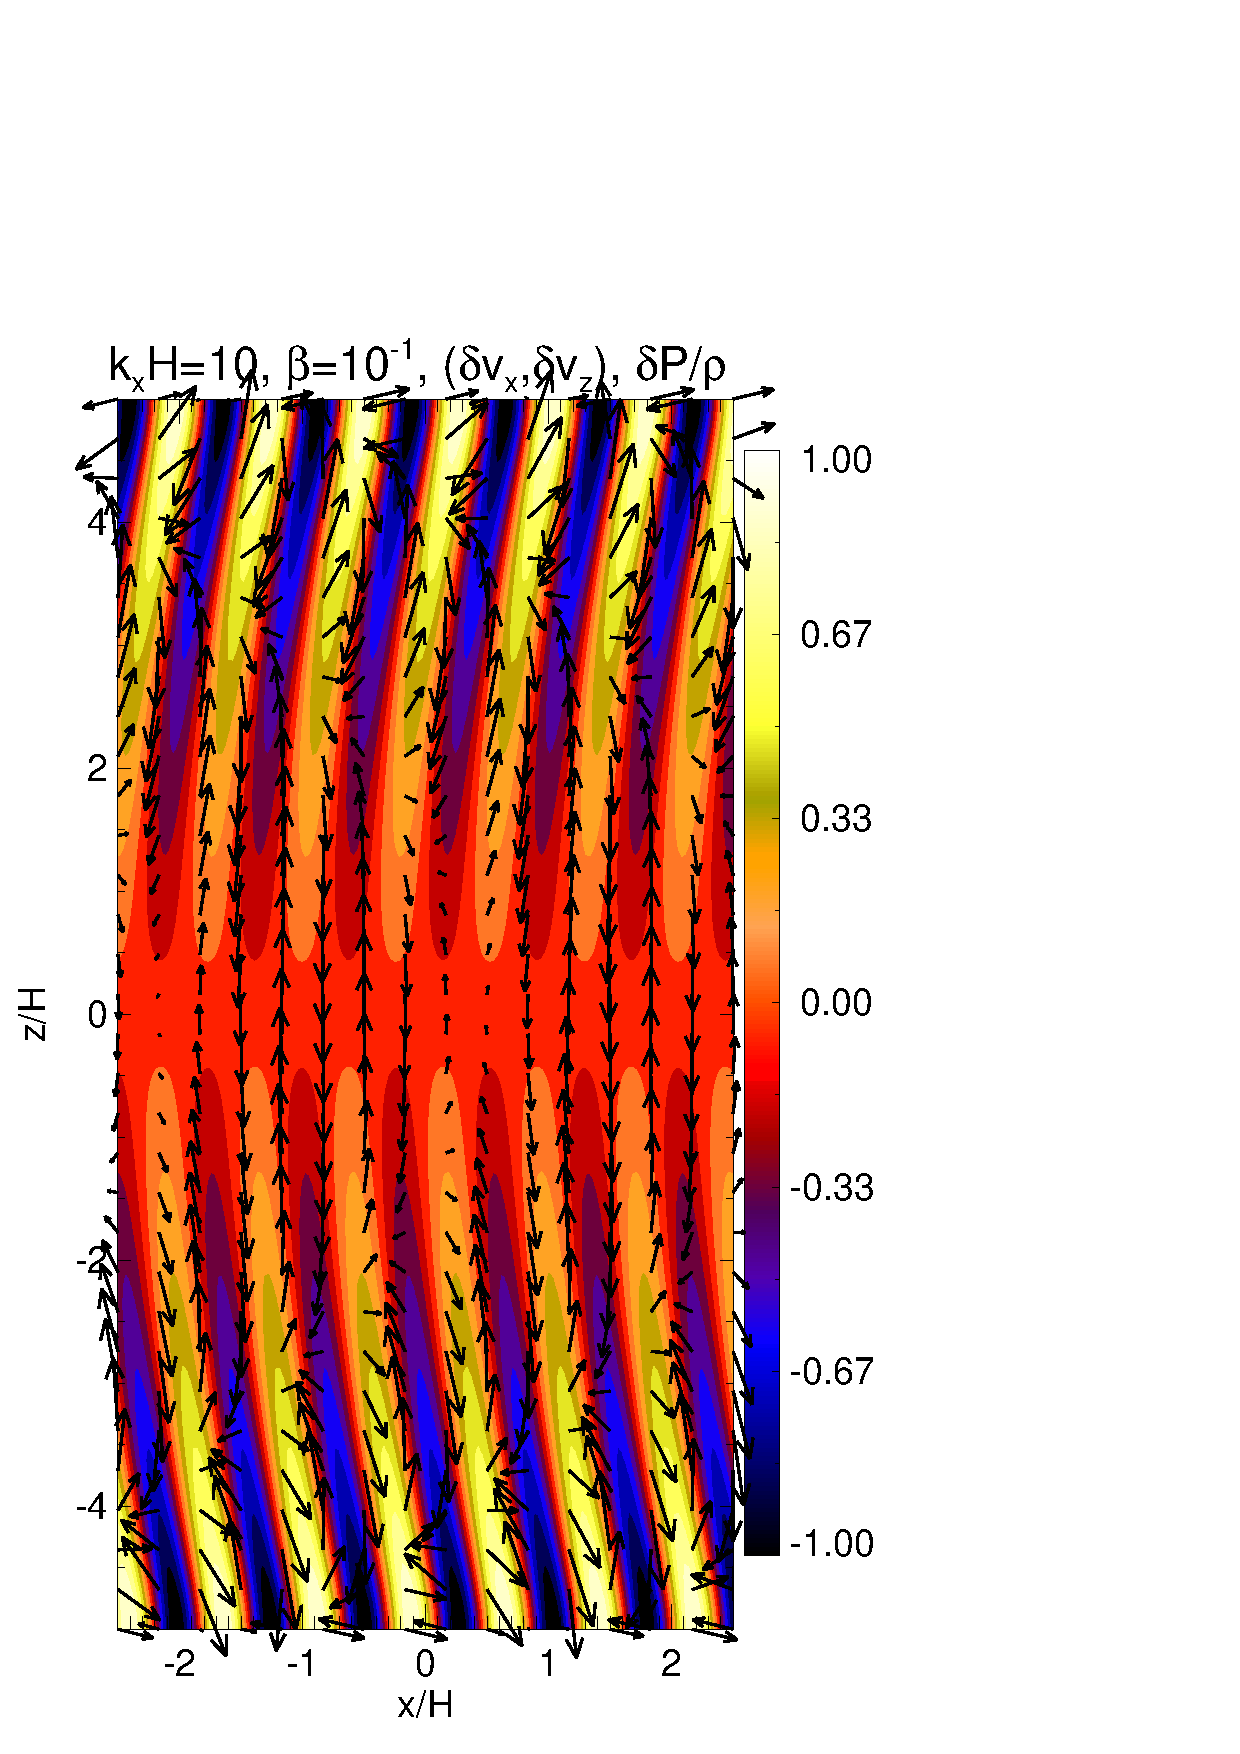
\includegraphics[scale=0.345,clip=true,trim=0cm 0cm 2.5cm
  % 0cm]{figures/result2d_vel_cool}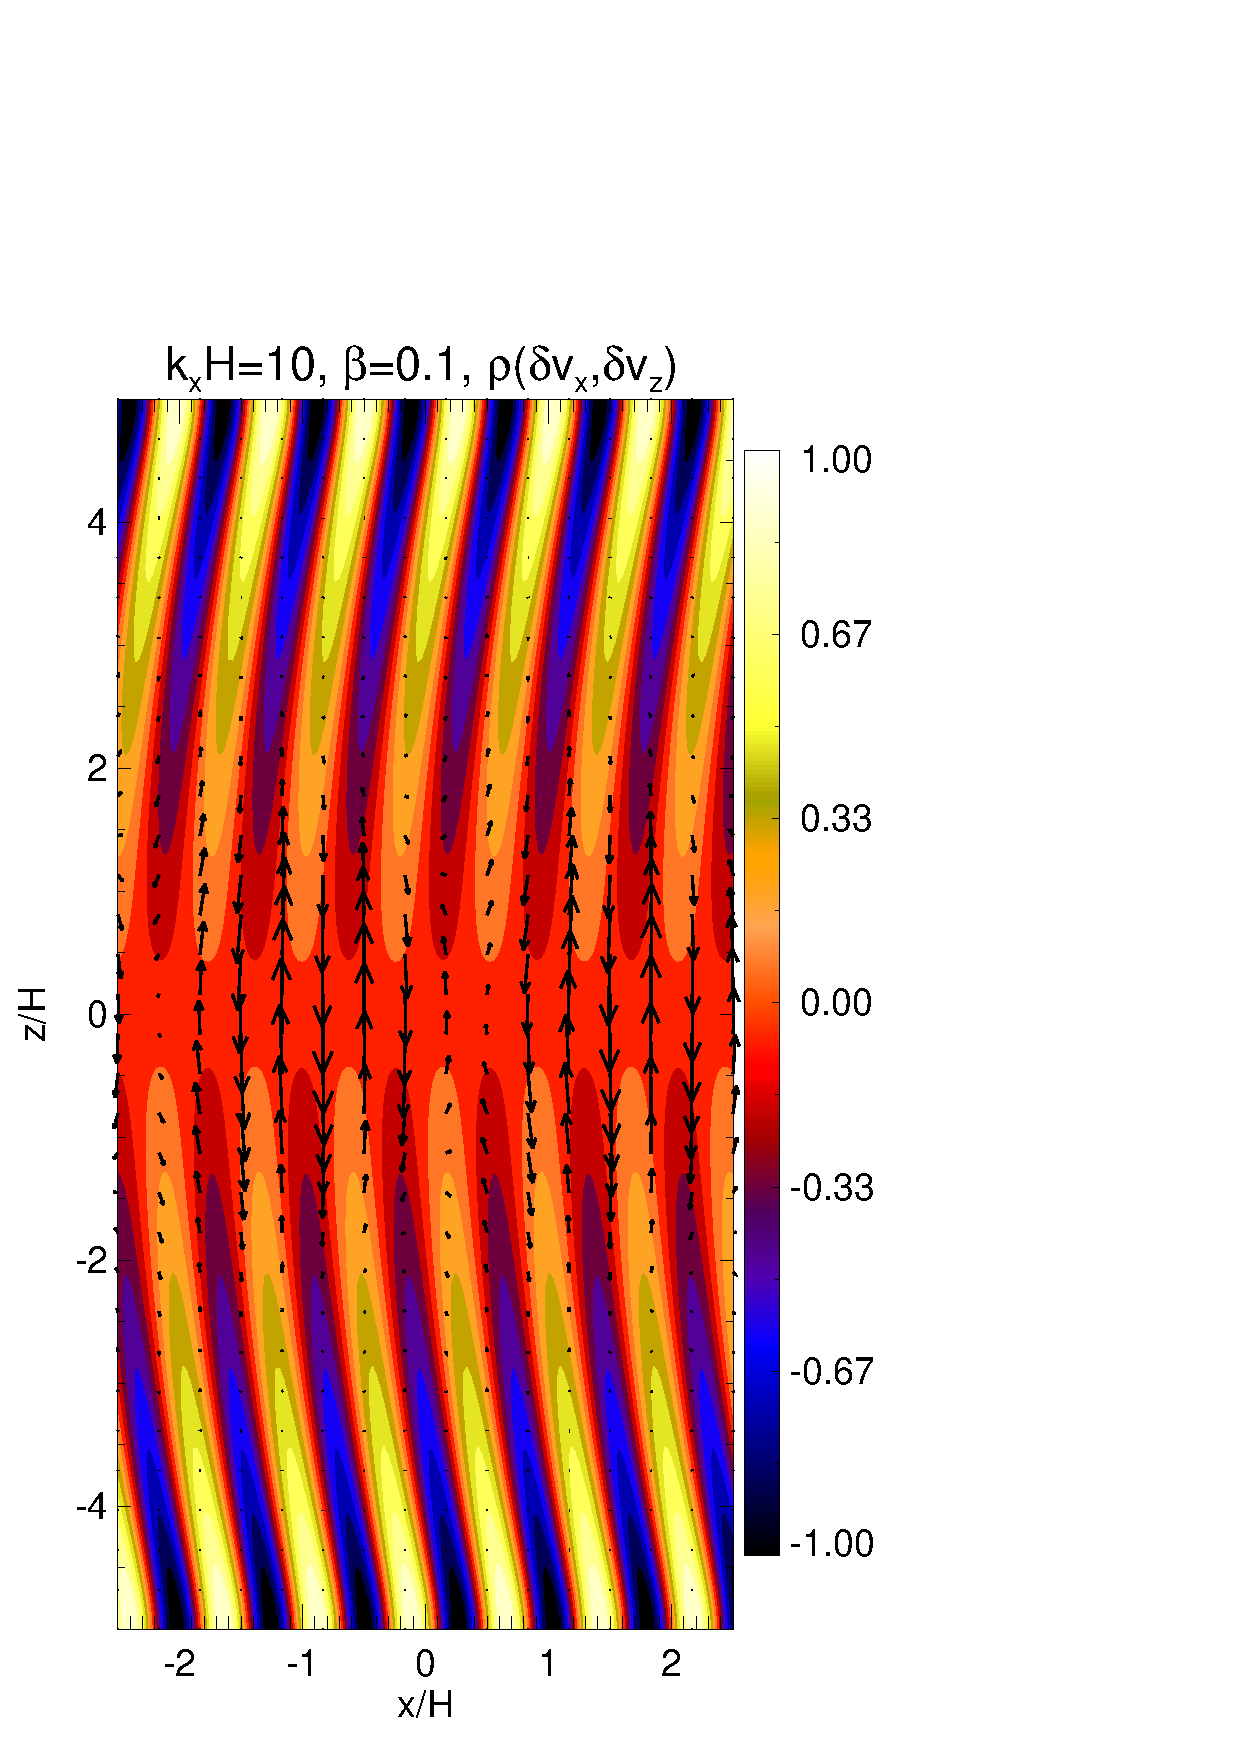
\includegraphics[scale=0.345,clip=true,trim=1.9cm 0cm 0cm
  % 0cm]{figures/result2d_mom_cool} 
  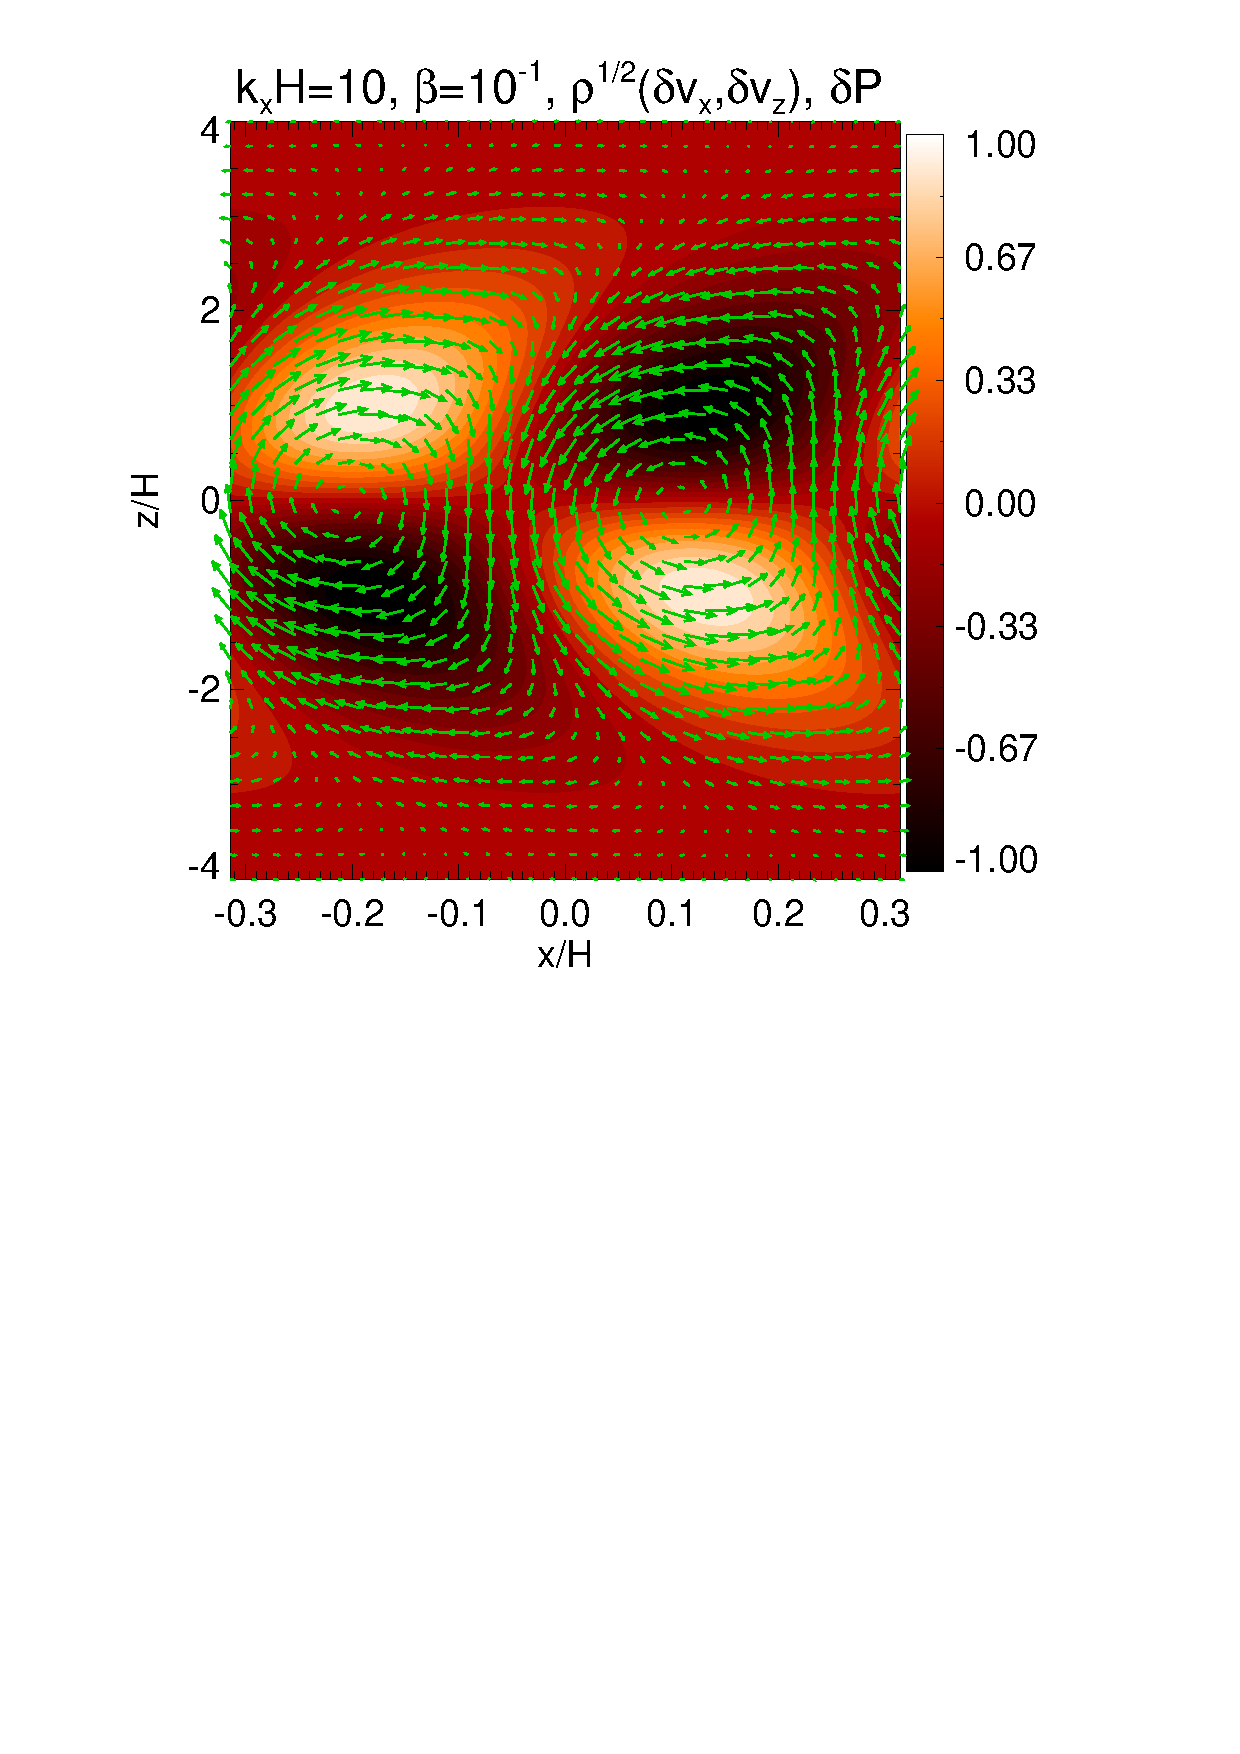
\includegraphics[width=\linewidth]{figures/result2d_cool}
  \caption{Same as  Fig. \ref{lowfreq_eigenfunc_2d} but with a thermal
    relaxation timescale $\beta=0.1$. 
    \label{lowfreq_eigenfunc_2d_cool}
  }
\end{figure}

In Fig. \ref{compare_modes_cool_kx30} we plot eigenvalues for unstable
modes with $\khat=30$. For clarity, we only plot analytic results 
for the fundamental mode ($M=0$) and $M=1,\,2$, and omit the
squares. The fundamental mode is again insensitive boundary
conditions compared to higher order modes, and are in close agreement
with analytic results. As before we observe more effective
stabilization for higher order modes, including the absence of surface
modes (which only occur for $\zmax\geq 5H$) as $\beta$ is increased.  
For $\zmax=3H$, the fundamental mode becomes dominant for $\beta\geq
0.03$. For $\zmax=5H$ and $\zmax=7H$, we
find modes slightly more unstable than the fundamental
mode even when $\beta=0.1$ (the leftmost eigenvalues in the lower two
panels), but these are likely associated  with the boundary
condition as they are absent for $\zmax=3H$. These observations
suggest the fundamental mode to be more robust in realistic disks.    

\begin{figure}
  \includegraphics[width=\linewidth,clip=true,trim=0cm 1.75cm 0cm
  0cm]{figures/compare_modes_cool_kx30_z3_analytic.ps} 
  \includegraphics[width=\linewidth,clip=true,trim=0cm 1.75cm 0cm
  0cm]{figures/compare_modes_cool_kx30_z5_analytic.ps}
  \includegraphics[width=\linewidth]{figures/compare_modes_cool_kx30_z7_analytic.ps}
  \caption{Same as Fig. \ref{compare_modes_cool_kx10} but for
    $\khat=30$. Examples of surface modes are marked with `s'. 
    \label{compare_modes_cool_kx30} 
  }
\end{figure}

Fig. \ref{compare_modes_cool_kx10} and \ref{compare_modes_cool_kx30} 
show that the fundamental mode is not sensitive to boundary
conditions. The fundamental mode also becomes dominant as $\beta$
approaches $\beta_\mathrm{crit}$, except with the possible emergence
of modes associated with boundary conditions. Thus, tracking the
fundamental mode is a more preferable assessment of stability as $\beta$
is increased from zero, rather than searching for the most unstable
mode, because the latter may correspond to modes that depend on boundary
conditions.   


%boundary conditions play an increasing role for higher M

\subsection{Critical thermal relaxation
  timescale}\label{bcrit_num_test}
We now test the critical thermal relaxation timescale given by
Eq. \ref{iso_vsi_cond}. We begin from eigenvalues for the fundamental
mode with $\beta=10^{-3}$ and slowly increase the thermal
relaxation timescale up to $\beta=10^3$. Fig. \ref{bcrit_compare1}
show the obtained growth rates, together with the critical  
thermal relaxation timescale $\beta_\mathrm{crit}=0.125$ for our
fiducial disk parameters.   

For $5\lesssim\khat\lesssim30$, we find $\beta_\mathrm{crit}$ provides
an accurate prediction of the upper limit to the thermal relaxation 
timescale for the fundamental mode. For smaller $\khat$, the VSI can
operate slightly beyond $\beta_\mathrm{crit}$ (recall that
$\beta_\mathrm{crit}$ was derived for $\khat^2\gg 1$). For
$\khat\geq 50$, we find perturbations have large amplitudes near the
 vertical boundaries, and 
complications to our numerical search of
eigenvalues arise from the emergence of modes associated with boundary
conditions. %We generally find boundary effects become more significant
%with increasing $\khat$.  
Nevertheless, growth rates rapidly decrease as $\beta$
approaches and increase beyond $\beta_\mathrm{crit}$.  

Fig. \ref{bcrit_compare1} is consistent with numerical simulations
performed by \cite{nelson13} for which a thermal relaxation timescale
$\beta\gtrsim 0.6$ stabilized the VSI. This can be anticipated from our
estimate of the critical thermal timescale $\beta_\mathrm{crit}\simeq
0.1$ for our fiducial disk parameters (which is the same as that
adopted by \citeauthor{nelson13}). It is interesting to note that there is a
thermal timescale that maximizes the mode decay rate. Here,
it is $\beta\simeq1$---$2$ or 
about $0.1$---$0.3$ orbital periods. This is in fact consistent with 
Fig. 12 of \cite{nelson13} where the perturbed kinetic energy in their
numerical simulations were observed to decay most rapidly for a
thermal timescale of $\sim 0.1$ orbits.     

\begin{figure}
   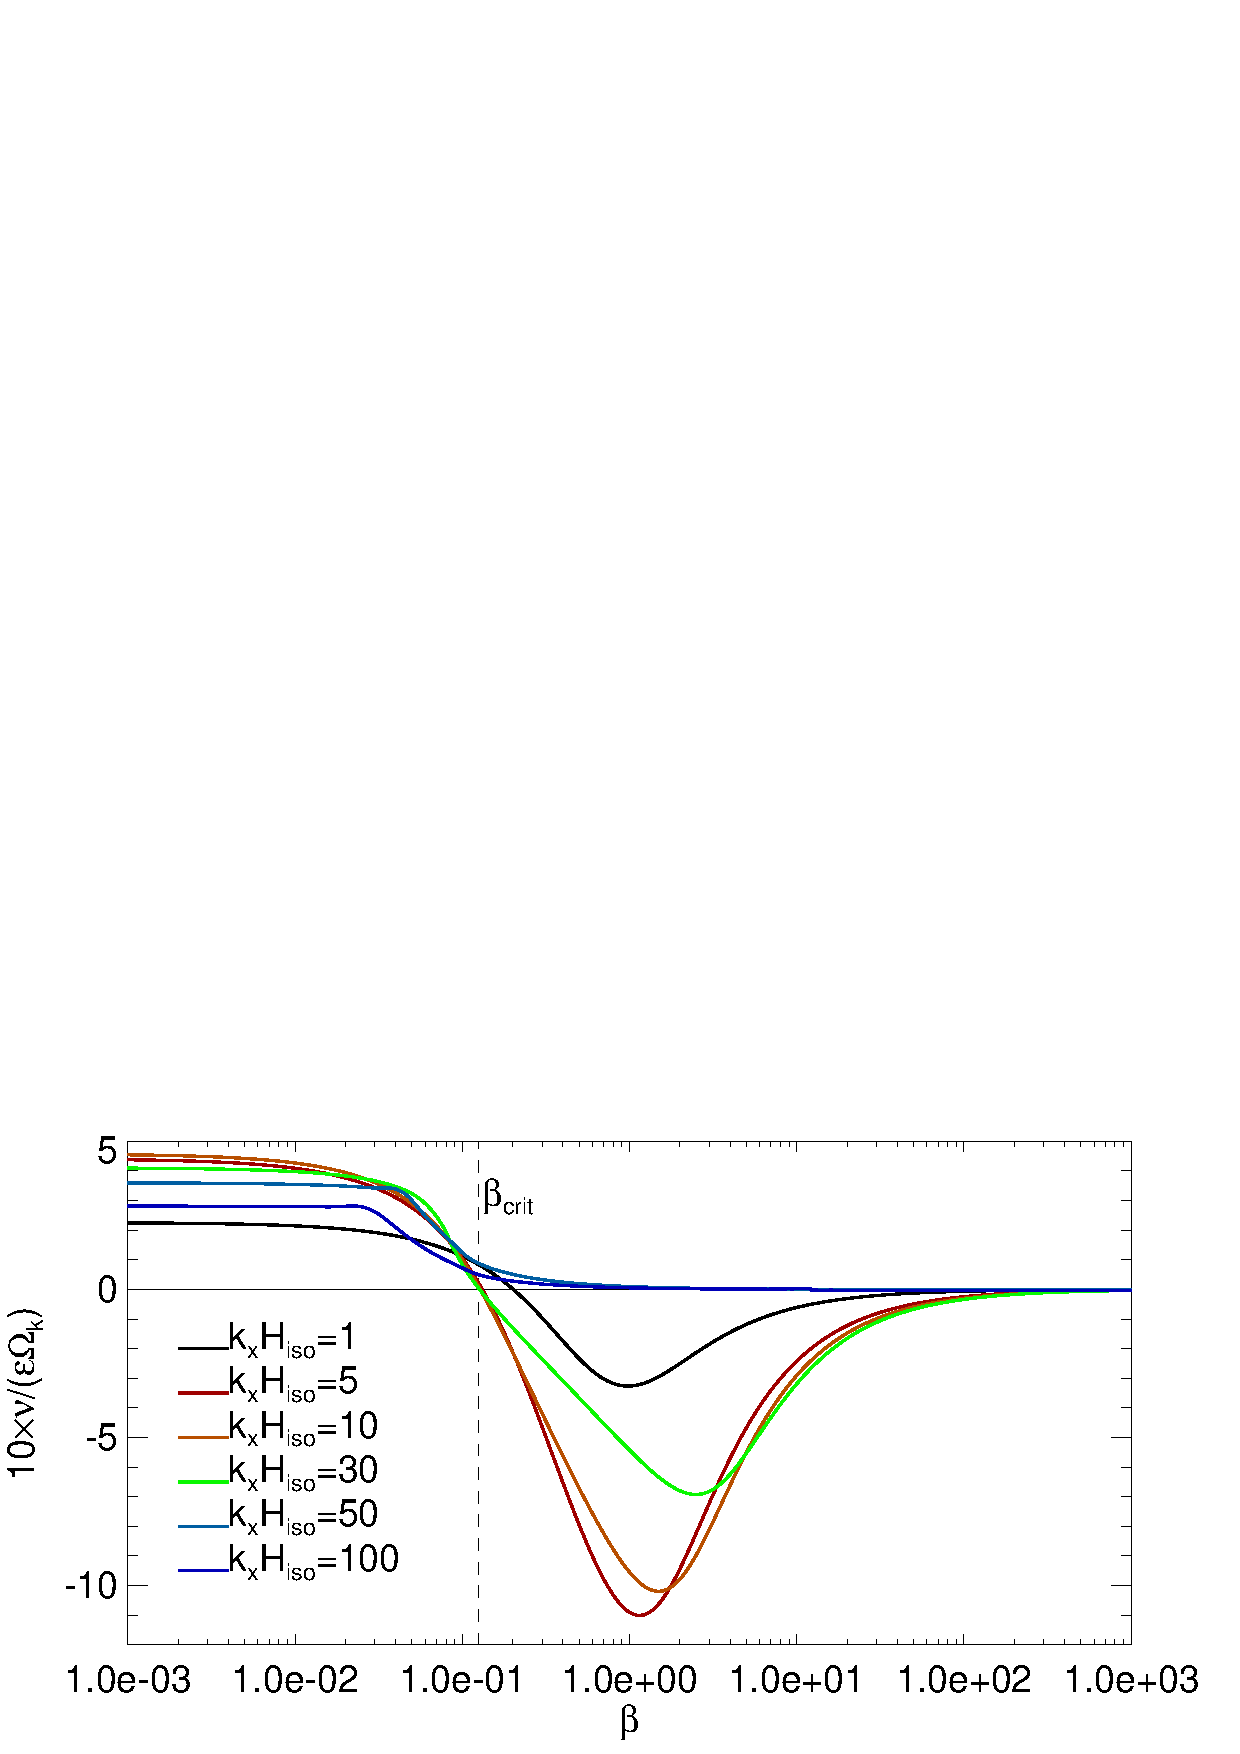
\includegraphics[width=\linewidth]{figures/gcorr_compare2} 
   \caption{VSI growth rates in the fiducial disk
     model as a function of the thermal relaxation timescale
     $\beta$. These are obtained by following the eigenvalues of the
     fundamental mode starting from $\beta=10^{-3}$ and increasing
     $\beta$. The vertical line is the
     critical thermal timescale $\beta_\mathrm{crit}$ obtained  
     from Eq. \ref{iso_vsi_cond}. 
     \label{bcrit_compare1}}   
 \end{figure} 
 
 We further test the dependence of the critical thermal relaxation timescale 
 $\beta_\mathrm{crit}$ on disk parameters (Eq. \ref{iso_vsi_cond}).
 We use the fiducial setup as a  reference point and vary
 $q\in[-0.2,-1.2]$,  $\gamma\in[1.2,2.0]$, and $\epsilon\in[0.02,0.1]$ 
 separately.

 The numerically obtained $\beta_\mathrm{crit}$ is shown in
 Fig. \ref{bcrit_compare} in comparison with Eq. \ref{iso_vsi_cond}.
 Our numerical results generally agree with Eq. \ref{iso_vsi_cond}. The
 agreement improves with decreasing  $|q|$,  $\epsilon$ and increasing
 $\gamma$, i.e. weaker instability. There is a noticeable difference
 as $\gamma\to1$ because the derivation of $\beta_\mathrm{crit}$
 assumed $\gamma>1$.   
 
 Fig. \ref{bcrit_compare}, together with Fig. \ref{bcrit_compare1} and 
 our finding that the fundamental mode becomes dominant as one
 increases $\beta$, and that it is not sensitive to boundary
 conditions, shows that $\beta_\mathrm{crit}$ as given  by
 Eq. \ref{iso_vsi_cond} provides a practical measure for the thermal
 relaxation timescale below which  VSI will operate. 

\begin{figure}
  \includegraphics[width=\linewidth,clip=true,trim=0cm 0.cm 0cm
  0cm]{figures/bcrit_compare_q.ps} 
  \includegraphics[width=\linewidth,clip=true,trim=0cm 0.0cm 0cm
  0.8cm]{figures/bcrit_compare_g.ps}
  \includegraphics[width=\linewidth,clip=true,trim=0cm 0.0cm 0cm
  0.8cm]{figures/bcrit_compare_e.ps} 
  \caption{Dependence of the upper limit to the thermal relaxation timescale
    $\beta_\mathrm{crit}$ for the fundamental VSI mode on disk
    parameters. Our fiducial setup is $(\gamma, \Gamma= (1.4, 1.011)$
    and $(p,q,\epsilon)=(-1.5,-1,0.05)$. Top: varying 
    $q\in[-1.2,-0.2]$; middle: varying $\gamma\in[1.2,2.0]$; bottom:
    varying $\epsilon\in[0.02,0.1]$. The perturbation wavenumber is
    $\khat=10$.  
    \label{bcrit_compare}}  
\end{figure}

\subsection{Vertically non-isothermal disks} 
We briefly consider vertically non-isothermal disks with 
$\Gamma=1.4$ and $(p,q,\epsilon)=(0,-1,0.05)$ as simulated in
\cite{nelson13}. In this case we set $\zmax=0.99H_s$.  

Fig. \ref{gcorr_compare_vnoniso} plots the fundamental VSI growth
rates as a function of $\beta$ for $\gamma\in[1.4,2.5]$. In agreement
with \citeauthor{nelson13}, in   
the neutrally-stratified case $\gamma=\Gamma$ the disk is unstable 
even for $\beta\gg 1$. This is due to the absence of a stabilizing
vertical entropy gradient ($N_z^2\equiv 0$). % (Note that in the adiabatic limit 
% this disk can be unstable according to the
% Solberg-Hoiland criterion, Eq. \ref{solberg2}.) 

For $\gamma>\Gamma$, i.e. stably stratified disks,
Fig. \ref{gcorr_compare_vnoniso} shows that introducing finite thermal
relaxation rapidly stabilizes the disk, similar to that observed for
nearly vertically isothermal disks (Fig. \ref{bcrit_compare1}). For
$\gamma=1.7,\,2.0,\,2.5$, growth rates reach zero at
$\beta\simeq0.17,\,0.083,\,0.045$, respectively. Interestingly, these
values are equal to $\epsilon|q|/(\gamma-\Gamma)$. This suggests that
the critical thermal relaxation timescale for vertically
non-isothermal disks can also be estimated by Eq. \ref{iso_vsi_cond}
but with $\gamma-1$ replaced by $\gamma-\Gamma$. 

\begin{figure}
  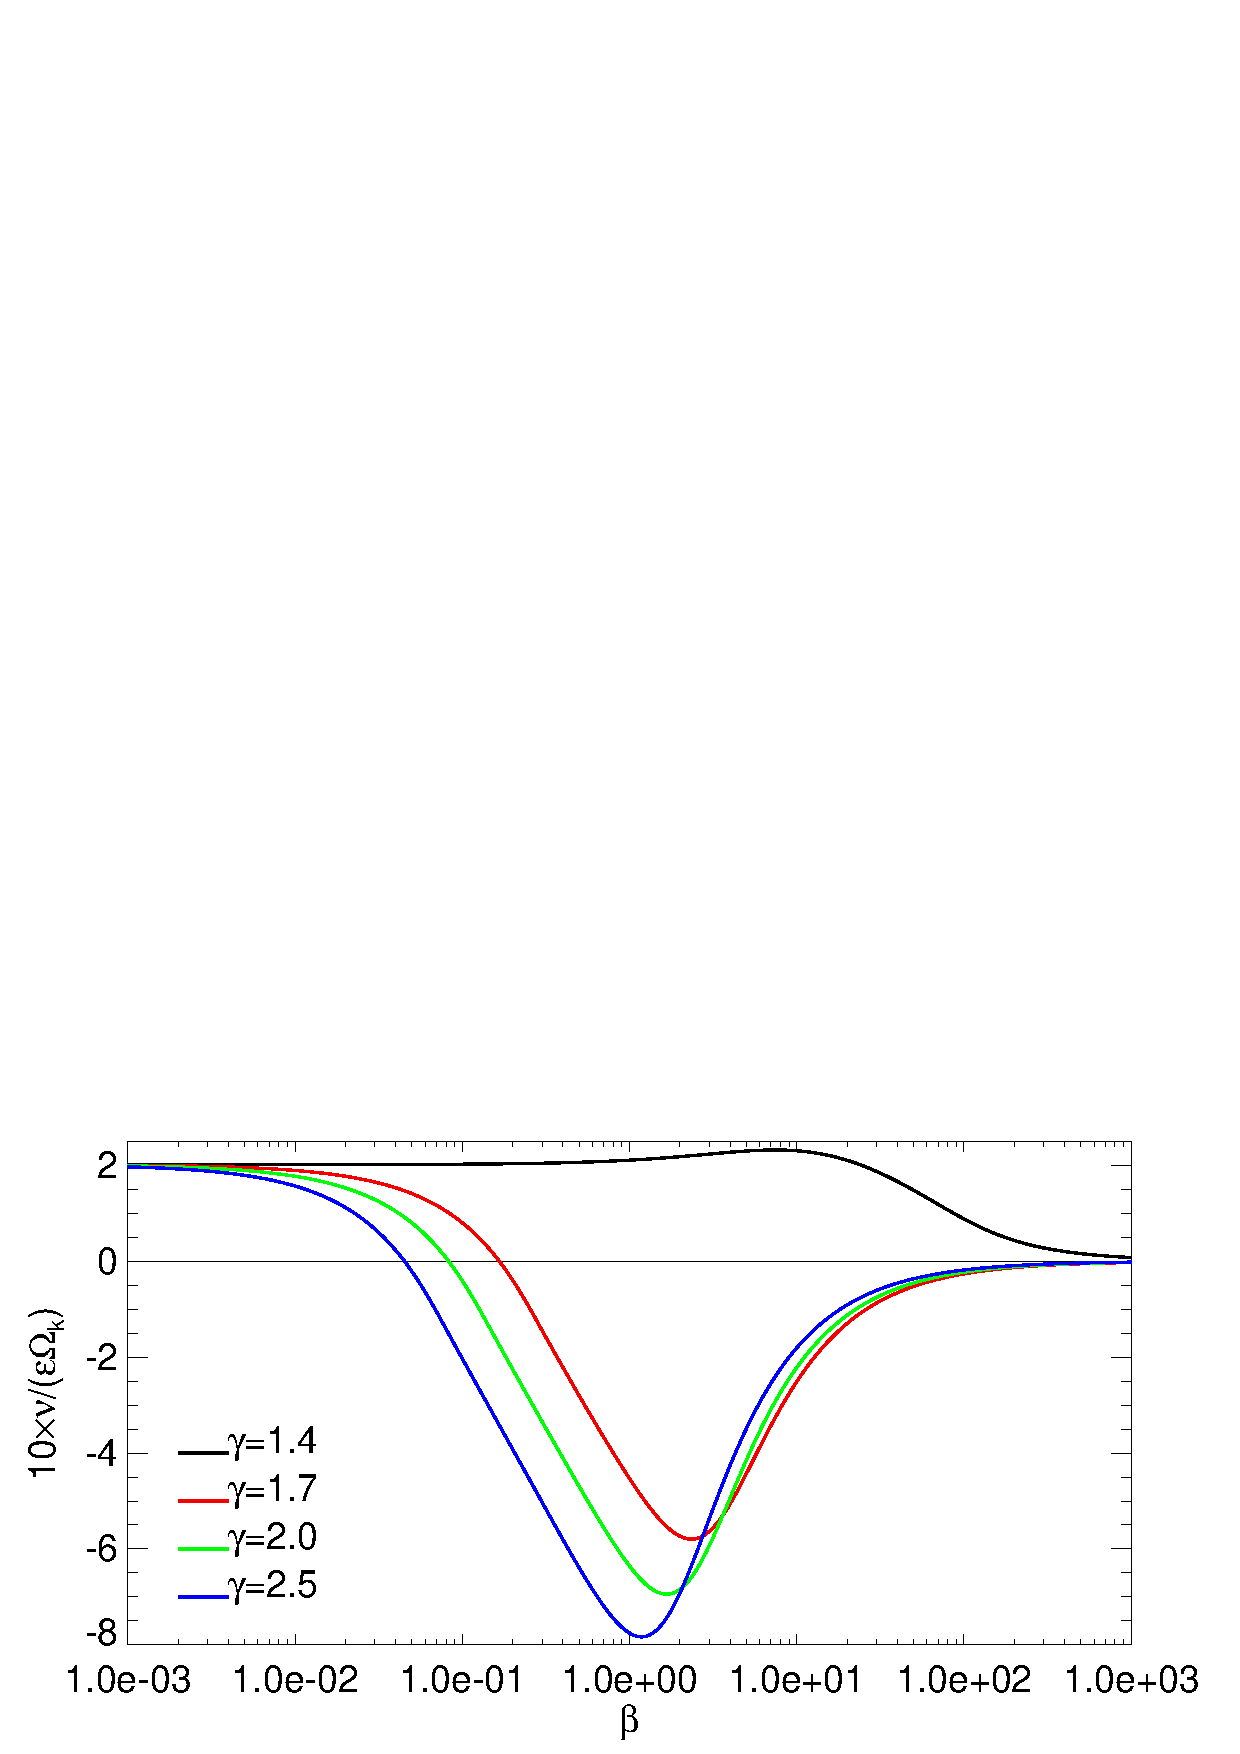
\includegraphics[width=\linewidth,clip=true,trim=0cm 0cm 0cm
  0cm]{figures/gcorr_compare_vnoniso2}
  \caption{Growth rate of the fundamental VSI mode as a function of
    the thermal relaxation timescale $\beta$, in vertically
    non-isothermal disks with $\Gamma=1.4$ and
    $\gamma\in[1.4,2.5]$. The disk is neutrally
    stratified for $\gamma=1.4$ and stably stratified for
    $\gamma>1.4$. Other disk parameters are
    $(p,q,\epsilon)=(0,-1,0.05)$ and the perturbation wavenumber is
    $\khat=30$.   
    \label{gcorr_compare_vnoniso}}
\end{figure}












